\begin{frame}
  \frametitle{Tipos de señales I}
  
  \centering
  \rotatebox[origin=c]{90}{\alert{\scriptsize \color{blue}Número de Fuentes o Canales\color{black}}}
  \begin{tabular}{>{\columncolor{lightgray}}ccc}
    \multicolumn{3}{c}{\alert{\scriptsize \color{blue}Número de variables independientes\color{black}}}\\ 
    \rowcolor{lightgray}
    & \color{blue}\small \alert{Unidimensional}  & \color{blue}\small  \alert{Multidimensional}\\
    \rotatebox{90}{\color{red}\small Escalar\color{black}}     & \parbox{3cm}{\centering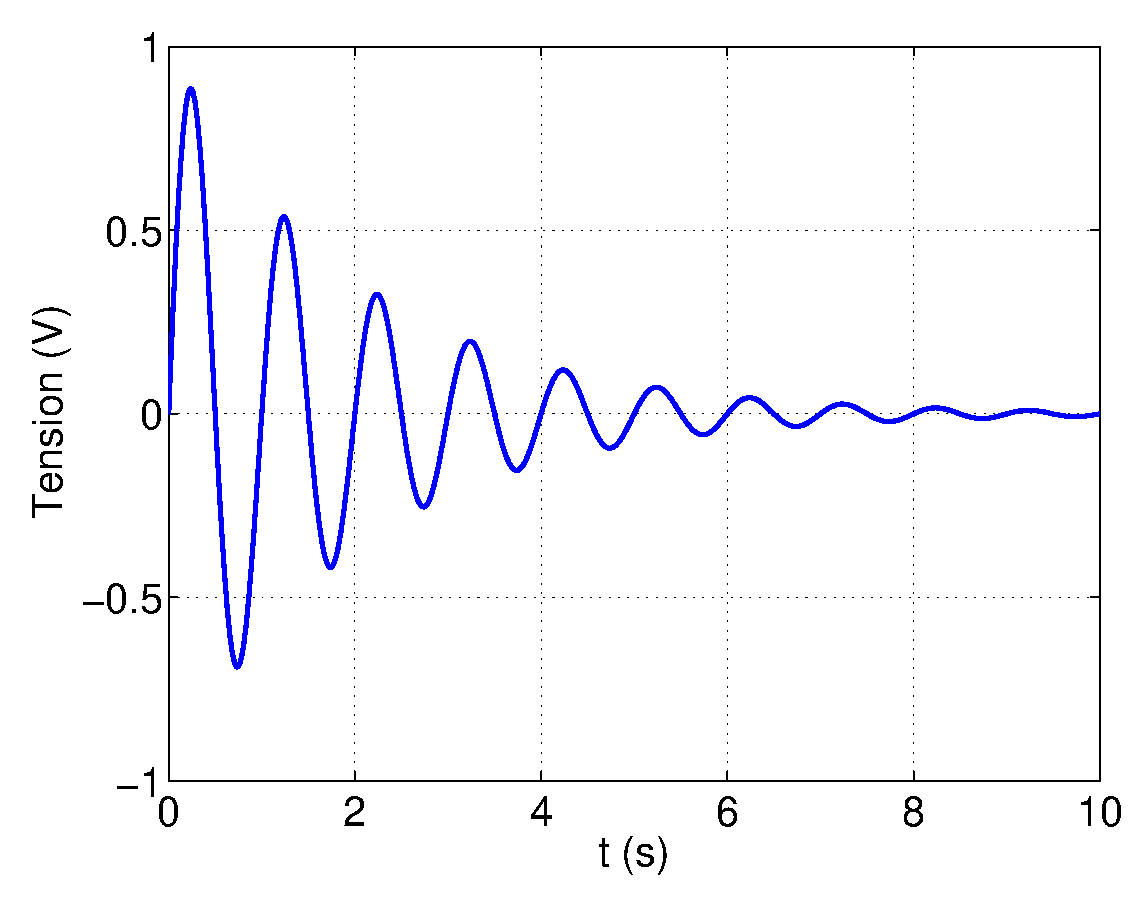
\includegraphics[height=2.4cm]{Figuras/UniScalar.eps}\\{\tiny $f(t)$}} & \parbox{3cm}{\centering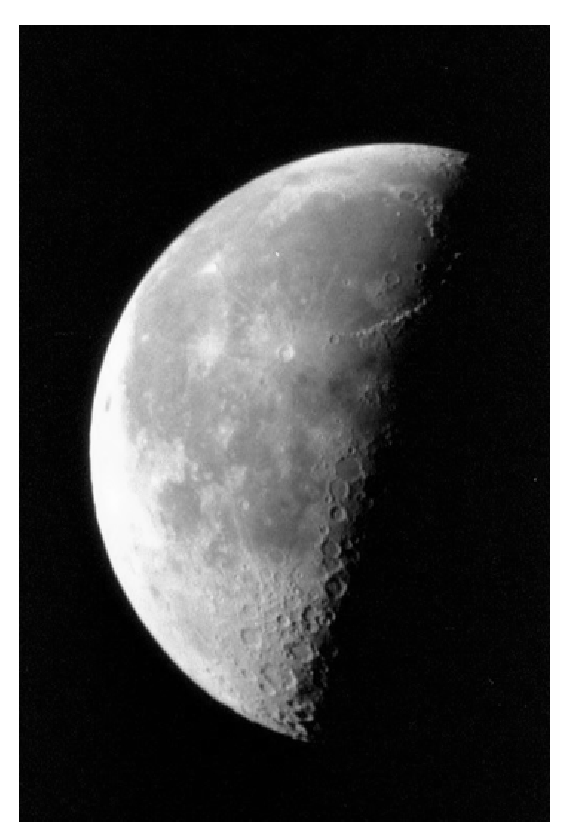
\includegraphics[height=2.3cm]{Figuras/Figures/ImagenBW.eps}\\{\tiny$f(x, y)$}} \\\\
    \rotatebox{90}{\color{red}\small Vectorial\color{black}}   & \parbox{4cm}{\centering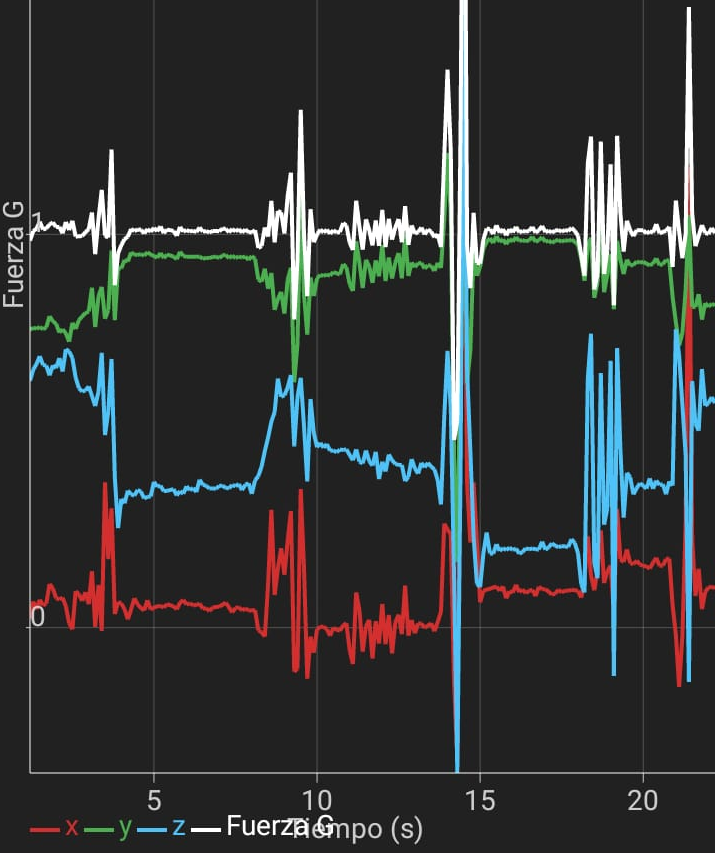
\includegraphics[width=2.0cm]{Figuras/UniVectorial.png}\\{\tiny$[f_x(t)~f_y(t)~f_z(t)~f_g(t)]$}} & \parbox{4cm}{\centering\includegraphics[height=2.3cm]{Figuras/Figures/ImagenColor.eps}\\{\tiny$[f_R(x, y)~f_G(x, y)~f_B(x, y)]$}} \\
  \end{tabular}
\end{frame}

% Basado en la presentación, aquí tienes ejemplos prácticos para 
% cada uno de los tipos de señales mencionados:

% 1. Según el número de fuentes o variables (Tipos I)
% Unidimensional: 


% Una señal de audio (voz), donde la presión acústica varía solo 

% en función del tiempo1111.


% Multidimensional: Una fotografía digital (imagen fija), que 
% varía en función de dos variables espaciales $(x, y)$

% 2222.Escalar: 
% La medición de la temperatura de una habitación a
%  lo largo del día3.
 
%  Vectorial: Una señal de vídeo en color (RGB),
 
%  donde en cada punto y momento se tienen tres componentes de 
%  intensidad (Rojo, Verde y Azul)
 
%  4444.2. 
%  Según la naturaleza de la variable y la amplitud (Tipos II)A
%  nalógica (Continua en tiempo y amplitud): 
%  La tensión eléctrica que sale directamente de un micrófono 
%  antes de ser procesada
 
%  5555.Muestreada (Discreta en tiempo, continua en amplitud): 
%  Los valores de esa tensión tomados a intervalos regulares, 
%  pero manteniendo su precisión decimal exacta antes de ser 
%  convertidos a bits
 
%  6.Digital (Discreta en tiempo y amplitud): 
%  Un archivo MP3 o un audio grabado en un CD, 
%  donde los valores ya están cuantizados en niveles definidos 
%  (bits)
%  7.3. 
 
%  Según su determinación (Tipos III)Determinista: Una señal de reloj de un procesador o un tono puro generado por un sintetizador ($x[n] = \sin(n)$), cuyo valor futuro es predecible8.Aleatoria / Estocástica: El ruido blanco (estática) de una radio sin sintonizar o las fluctuaciones del mercado de valores, que solo pueden describirse mediante probabilidades9.4. Según su repetición y simetría (Tipos IV y V)Periódica: La señal de la red eléctrica (50Hz/60Hz), que repite su forma de onda senoidal constantemente10.Aperiódica: Un golpe de tambor único o una palabra suelta, que no se repiten de forma infinita11.Par: Una señal de pulso rectangular centrado en el origen $t=0$12121212.Impar: Una señal de onda senoidal $(\sin(t))$, que es simétrica respecto al origen13131313.5. Según su relación con el tiempo (Tipos VI)Causal: Cualquier sistema físico real en funcionamiento, como un sensor que empieza a registrar datos solo después de encenderse (vale 0 para $t < 0$)14.Anticausal: Se utiliza principalmente en procesado de archivos grabados (post-procesamiento), donde podemos analizar la señal "hacia atrás" desde el presente hacia el pasado15.6. Según su energía y potencia (Tipos VII y VIII)De Energía Finita: Un pulso único o un transitorio que desaparece rápidamente; tiene una duración limitada16.De Potencia Finita: Una onda senoidal infinita o el ruido constante de un motor; aunque duran para siempre, su promedio de energía por unidad de tiempo es constante17.7. Señales Básicas de la PresentaciónImpulso ($\delta$ de Dirac): El modelo matemático de un martillazo instantáneo o un destello de flash fotográfico18.Escalón ($u(t)$): El acto de encender un interruptor, donde la tensión pasa de 0 a un valor constante instantáneamente19.Chirp: El sonido que emiten los radares o los delfines, cuya frecuencia aumenta o disminuye con el tiempo20.





\begin{frame}
  \frametitle{Tipos de señales II}
  \vspace{-0.1cm}
  \begin{itemize}
    \item <1-> Respecto a la variable independiente:
    \begin{itemize}
      \vspace{0.1cm}
      \item \alert{Continua}: $x(t)$ con $t\in \mathbb{R} $ (real)
      \vspace{0.1cm}
      \item \alert{Discreta}: $x(n)$ (o secuencia x[n]) con $n\in \mathbb{Z}$ (entero)
    \end{itemize}
    \vspace{0.2cm}
    \item <2-> Respecto a la amplitud $x(\cdot)$ de la señal:
    \begin{columns}[T]
      \visible<1->{\begin{column}{4.6cm}
      \begin{itemize}
        \vspace{0.0cm}
        \item $x(\cdot) \in \mathbb{R}$  \color{gray}{(a $x(\cdot) \in \mathbb{C}$)}\color{black}
        \begin{itemize}
          \vspace{0.1cm}
          \item  $x(t) \rightarrow$ \alert{Analógica}
          \vspace{0.1cm}
          \item $x[n] \rightarrow$ \alert{Muestreada}
        \end{itemize}
        \vspace{0.2cm}
        \item  $x(\cdot) \in S$ discreto:
        \begin{itemize}
          \vspace{0.1cm}
          \item  $x(t) \rightarrow$ \alert{Cuantizada}
          \vspace{0.1cm}
          \item $x[n] \rightarrow$ \alert{Digital}
        \end{itemize}
        \vspace{0.1cm}
        \color{gray} { Ej: $ S\!=\! \{\!a\!+\!b\!\cdot \!k | k \!\in \! \mathbb{Z}\}$}
      \end{itemize}
    \end{column}}
    \hspace{-0.5cm} \visible<1->{\begin{column}{6cm}
    \begin{figure}
      \centering
      \footnotesize
      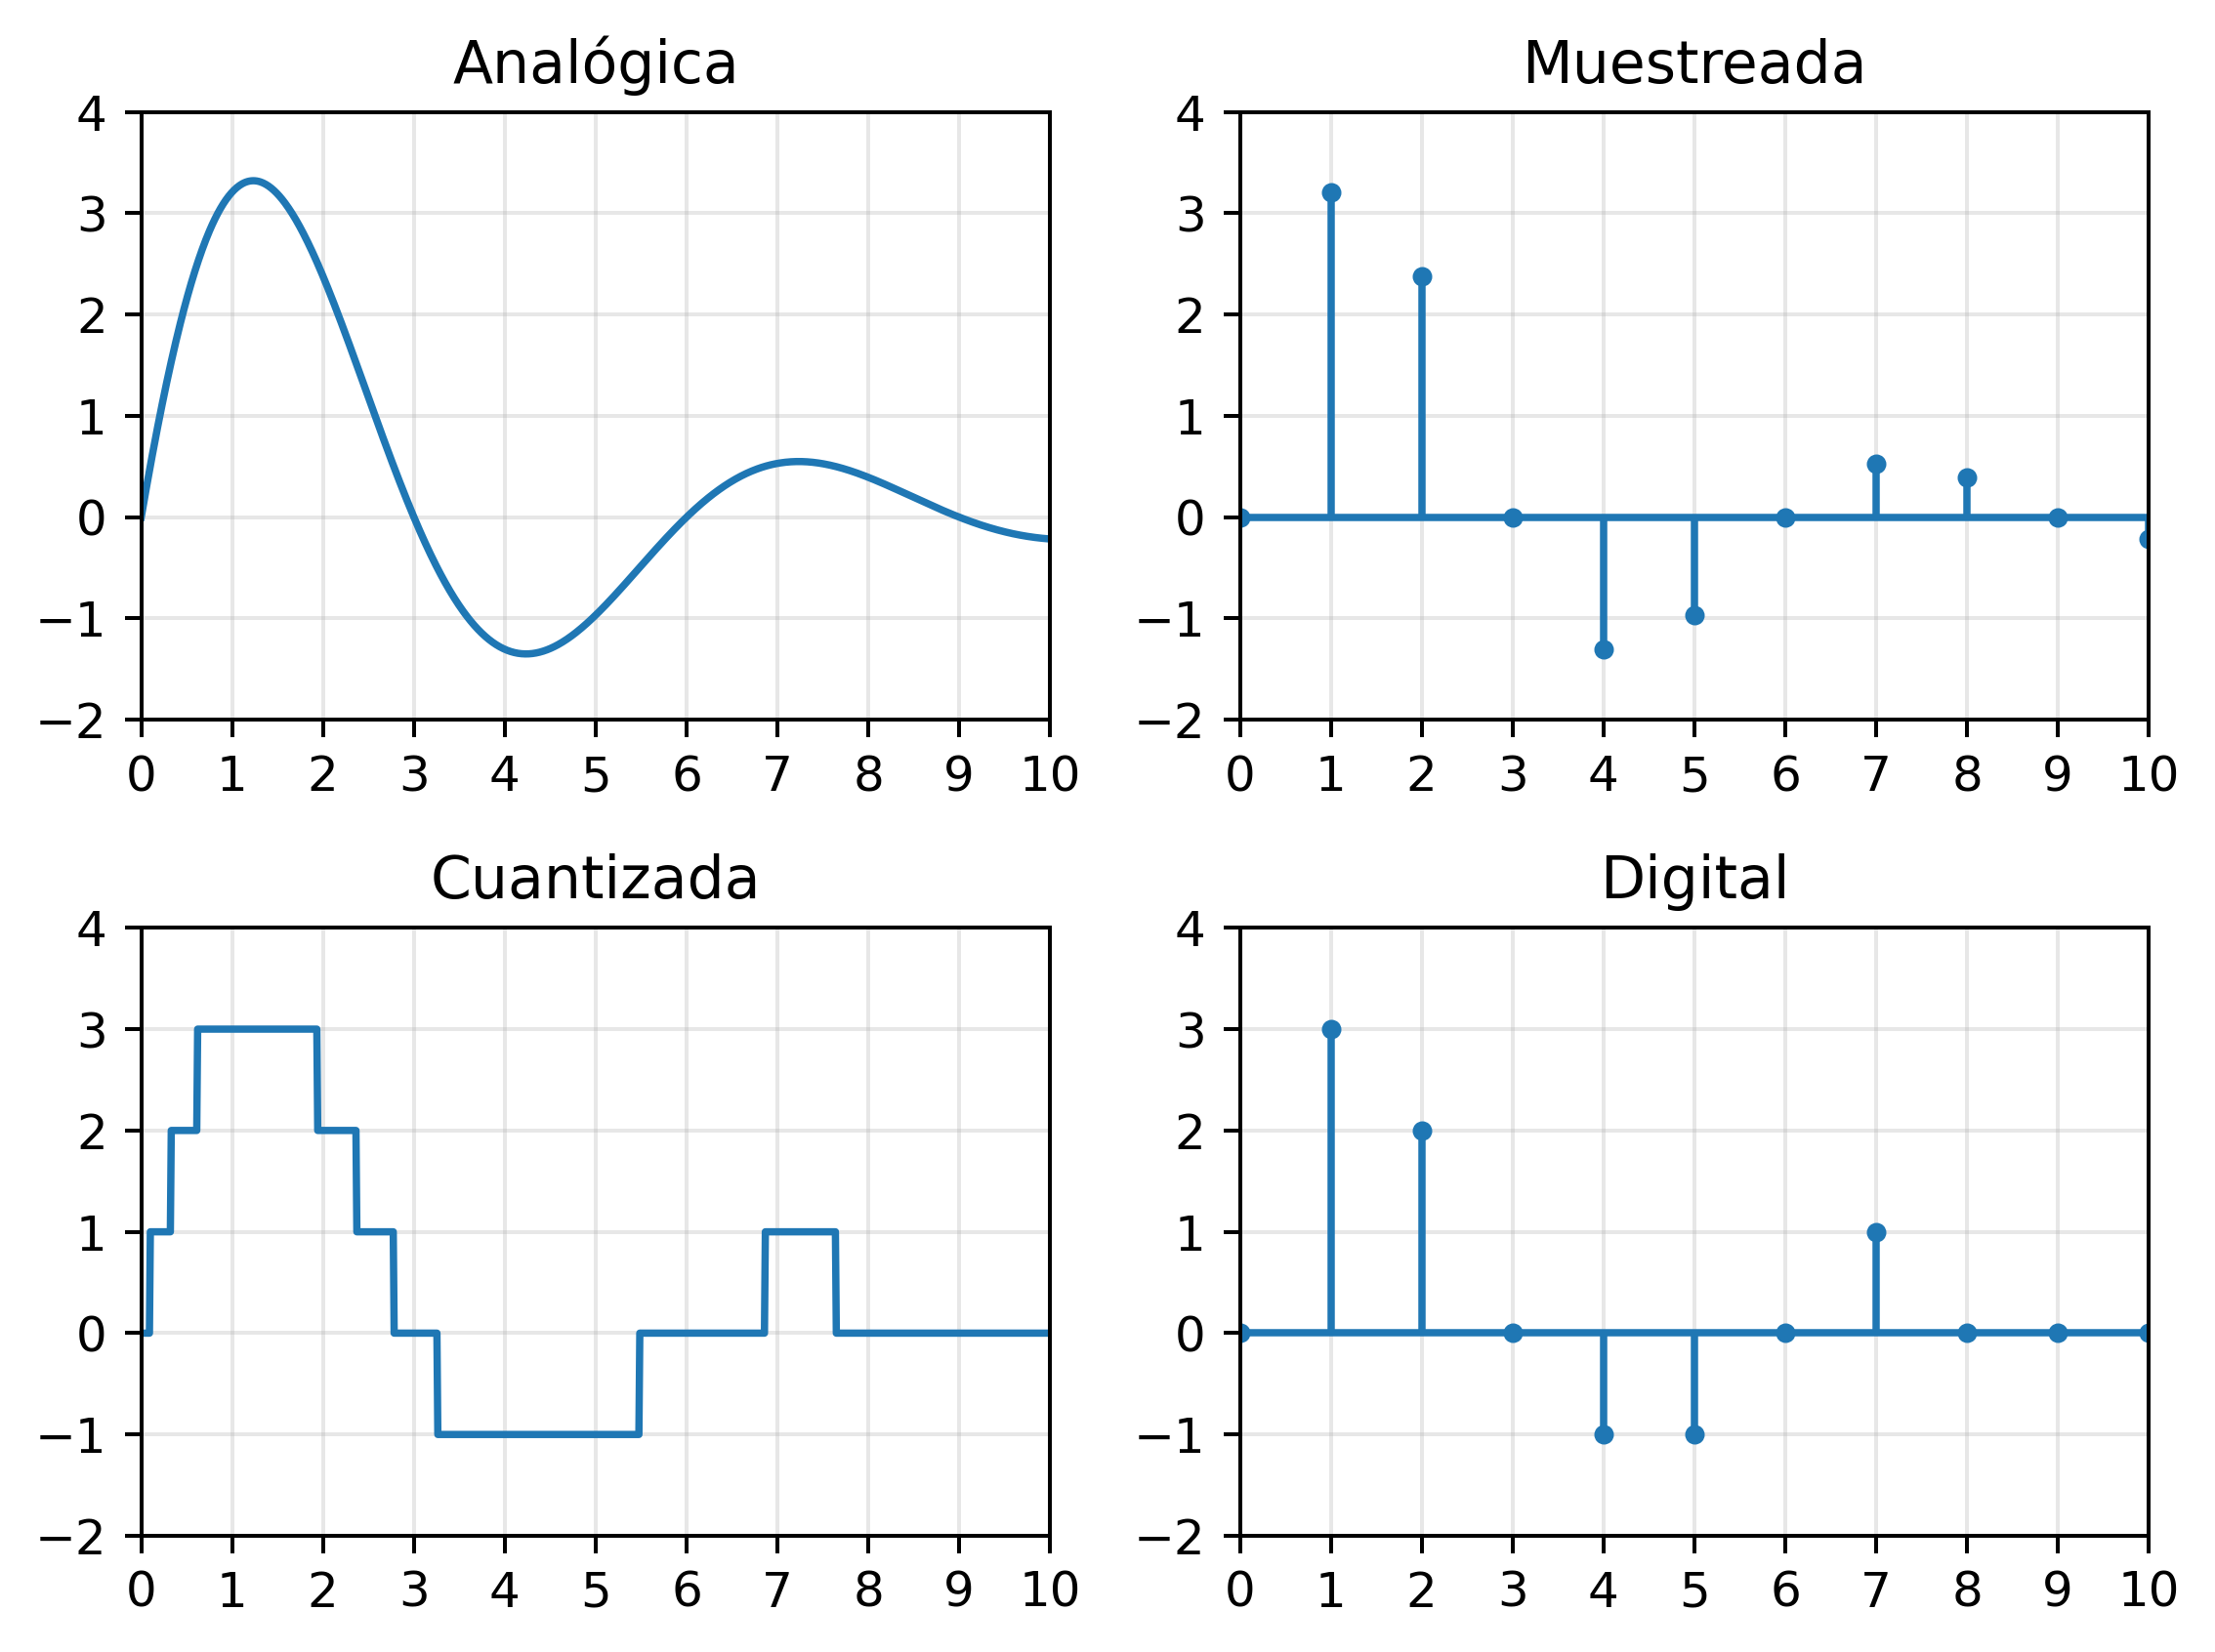
\includegraphics[width=6cm]{Figuras/ad.png}
    \end{figure}
    \end{column}}
  \end{columns}
  \end{itemize}
  \vspace{-0.5cm}
\end{frame}


\begin{frame}
  \frametitle{Tipos de señales III}
  \vspace{-0.1cm}
  \begin{itemize}
    \item <1-> Evolución de la señal (valor en cada instante de tiempo):
    \begin{itemize}
      \vspace{0.1cm}
      \item \alert{Determinista}:  está definido por una expresión matemática
      \vspace{0.1cm}
      \item \alert{Aleatoria/Estocástica}:  queda definido por una densidad de probabilidad (no se puede determinar de forma exacta).
    \end{itemize}
  \end{itemize}
  \vspace{-0.3cm}
  \begin{figure}
    \centering
    \footnotesize
    \begin{tabular}{@{\extracolsep{-8pt}}cc}
      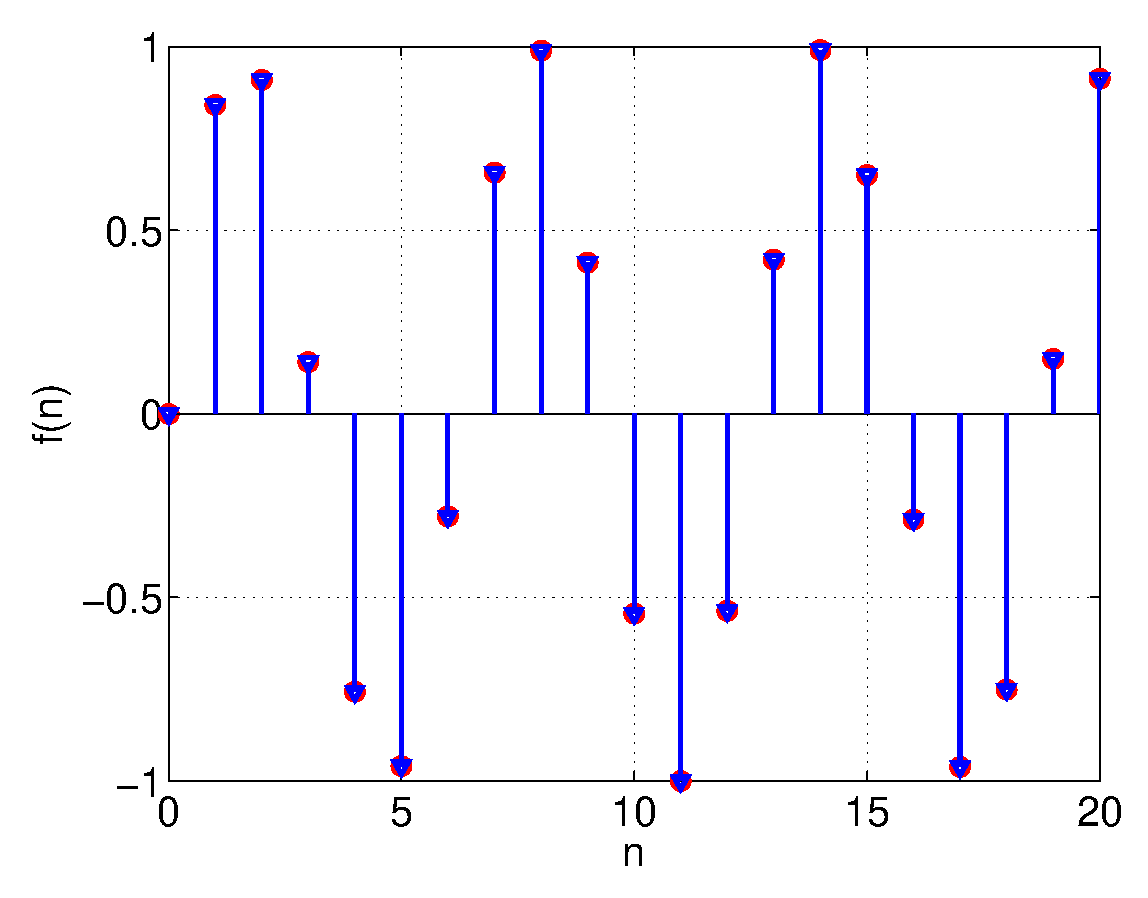
\includegraphics[width=5cm]{./Figuras/Determinista.eps}&
      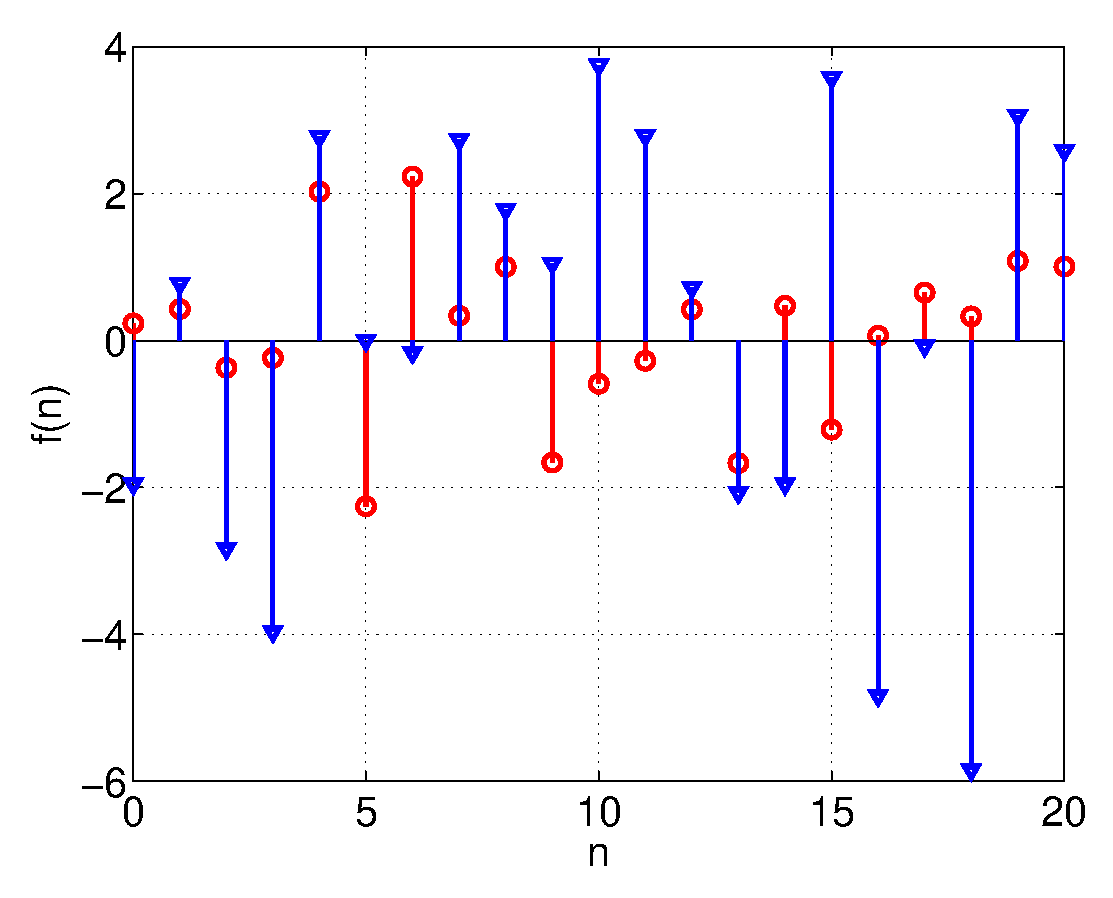
\includegraphics[width=5cm]{./Figuras/Aleatorio.eps}\\
      Determinista  & Aleatoria \\
      $x[n]=sin(n)$ & $x[n] \sim \mathcal{N}(0,1) $
    \end{tabular}
  \end{figure}
\end{frame}

\begin{frame}
  \frametitle{Tipos de señales IV}
  \vspace{-0.1cm}
  \begin{itemize}
    \item <1-> Señales periódicas/aperiódicas:
    \begin{itemize}
      \vspace{0.1cm}
      \item \alert{Periódica}: su valor se repite en el tiempo, por lo tanto es suficiente especificar su valor a lo largo de un intervalo básico llamado periodo fundamental ($T$ o $N$).
      \begin{itemize}
        \vspace{0.1cm}
        \item Continua: $x(t+l\cdot T)=x(t)$
        \vspace{0.1cm}
        \item  Discreta: $x[n+l\cdot N]=x[n]$
        \vspace{0.1cm}
        con $l \in \mathbb{Z}^+$,  $N \in \mathbb{Z}^+$
      \end{itemize}
      \vspace{0.1cm}
      \item \alert{Aperiódica}:  no cumple la relación anterior.
    \end{itemize}
  \end{itemize}
  \vspace{-0.3cm}
  \begin{figure}
    \centering
    \footnotesize
    \begin{tabular}{@{\extracolsep{-8pt}}cc}
      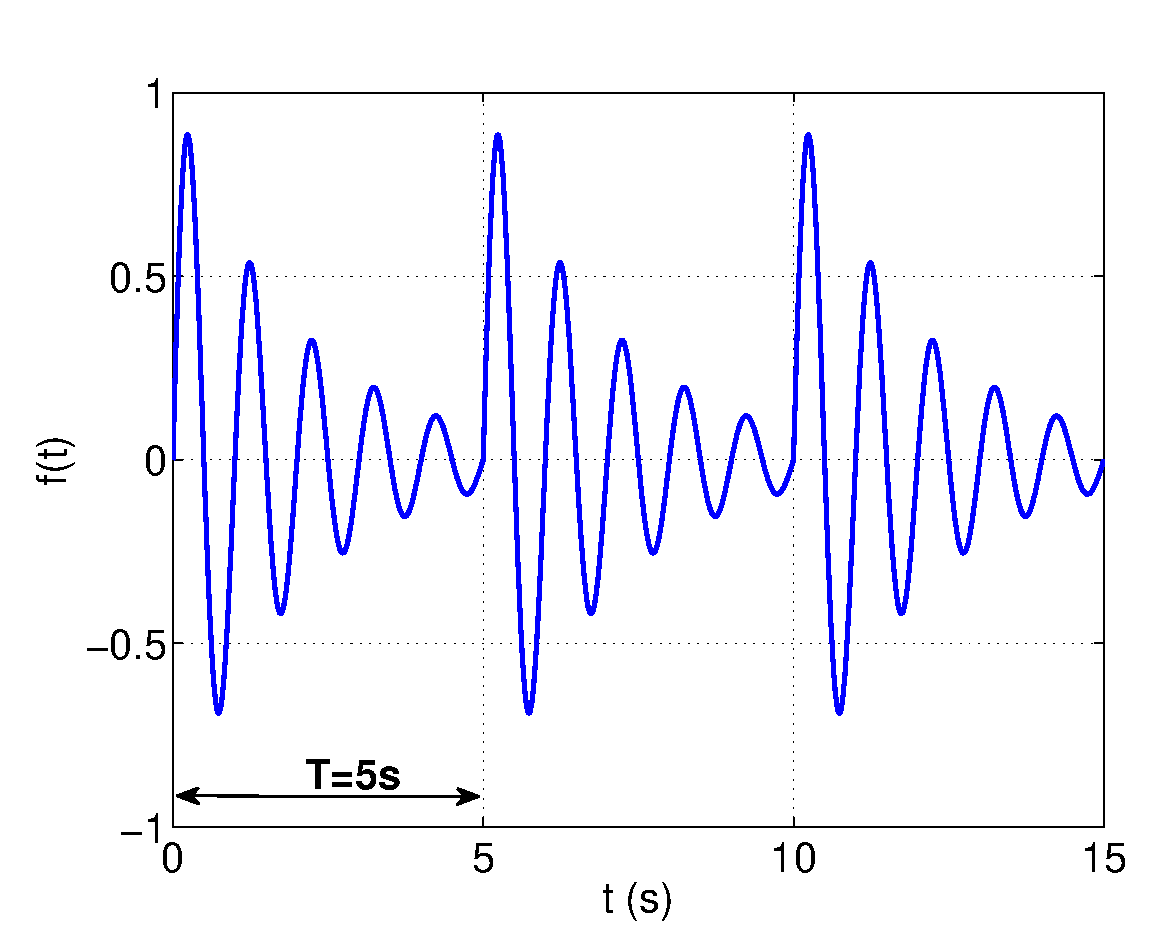
\includegraphics[width=5cm]{./Figuras/PeriodT.eps}&
      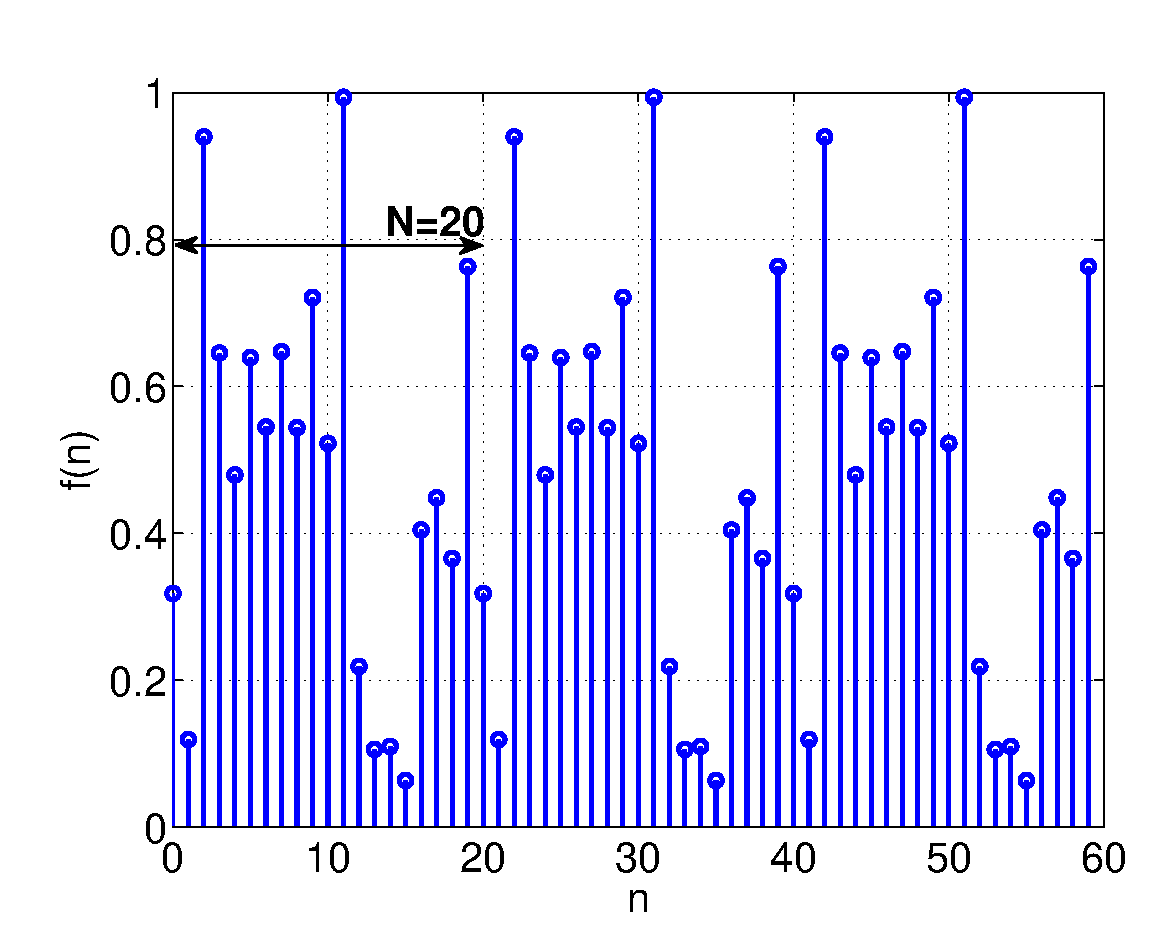
\includegraphics[width=5cm]{./Figuras/PeriodN.eps}\\
    \end{tabular}
  \end{figure}
\end{frame}

\begin{frame}
  \frametitle{Tipos de señales V}
  \vspace{-0.2cm}
  \begin{itemize}
    \item <1-> Señales pares/impares:
    \begin{itemize}
      \vspace{0.1cm}
      \item \alert{Par}: presenta simetría especular respecto a eje vertical.
      \vspace{0.1cm}
      \begin{itemize}
        \begin{columns}[c]
          \hspace{1cm}\begin{column}{3.8cm}
          \vspace{-0.15cm}
          \item Continua: $x(t)=x(-t)$
          \end{column}
          \hspace{-1.5cm}\begin{column}{3.8cm}
          \item  Discreta: $x[n]=x[-n]$
        \end{column}
      \end{columns}
    \end{itemize}
    \vspace{0.1cm}
    \item \alert{Impar}: presenta simetría radial respecto al origen.
    \vspace{0.1cm}
    \begin{itemize}
      \begin{columns}[c]
        \hspace{1cm}\begin{column}{3.8cm}
          \vspace{-0.15cm}
          \item Continua: $x(t)=-x(-t)$
        \end{column}
        \hspace{-1.5cm}\begin{column}{3.8cm}
          \item  Discreta: $x[n]=-x[-n]$
        \end{column}
      \end{columns}
    \end{itemize}
    \vspace{0.1cm}
    \vspace{0.1cm}
    \end{itemize}
  \end{itemize}
  \vspace{-0.75cm}
  \begin{figure}
    \centering
    \footnotesize
    \begin{tabular}{@{\extracolsep{-8pt}}cc}
      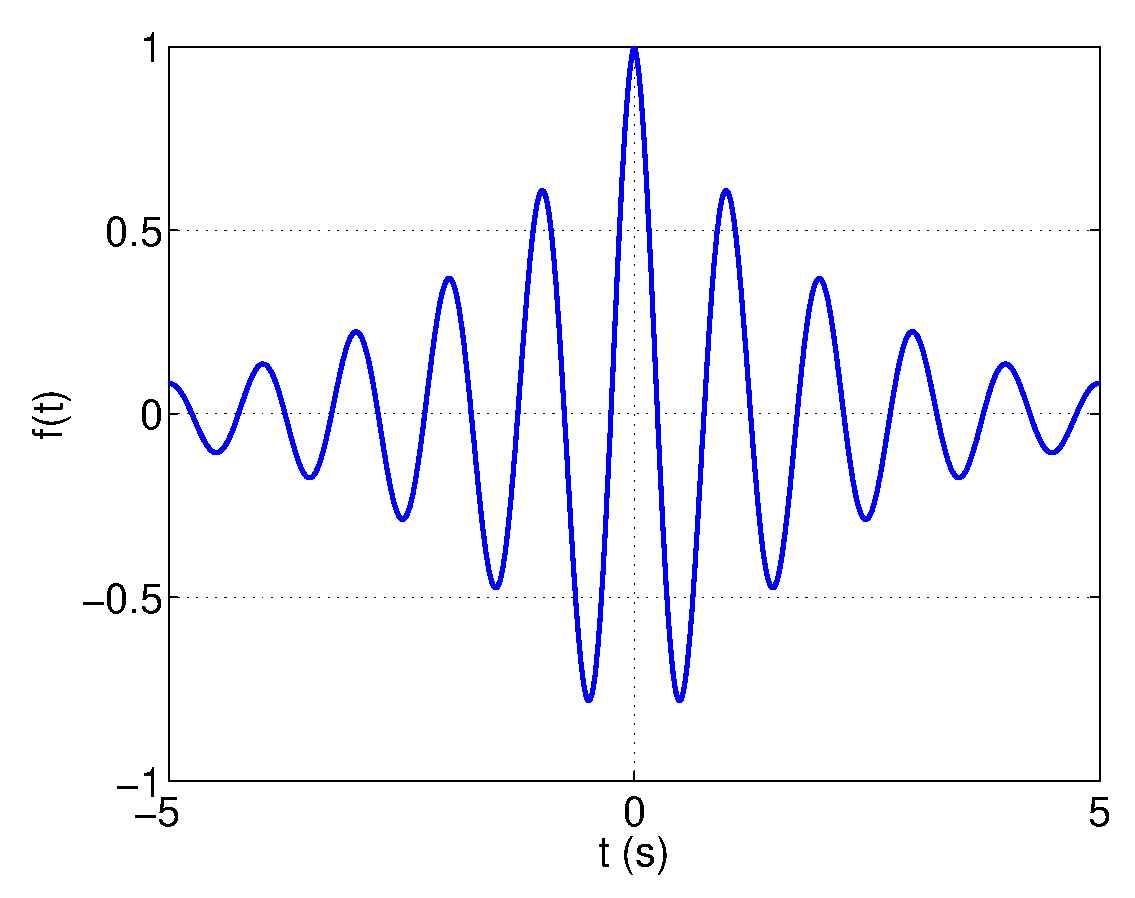
\includegraphics[width=4cm]{./Figuras/Par.eps}&
      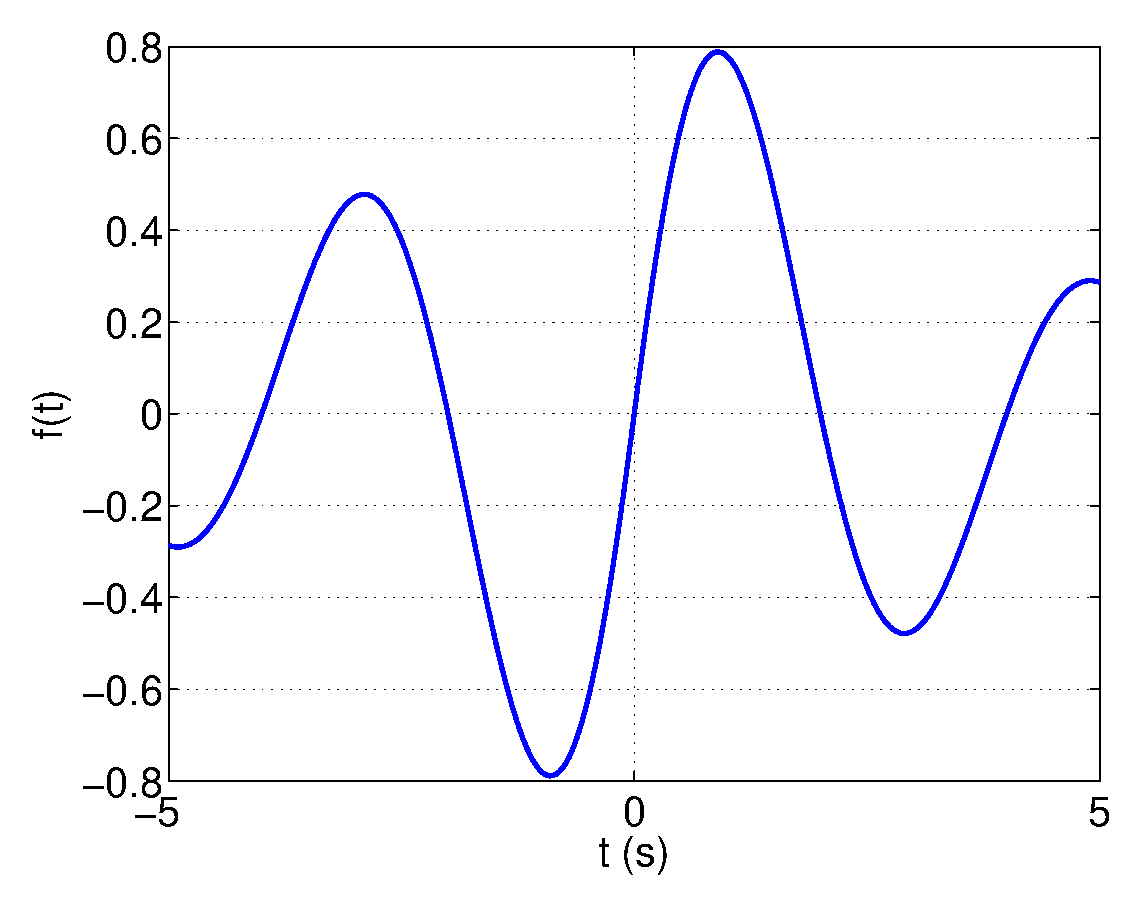
\includegraphics[width=4cm]{./Figuras/Impar.eps}\\
      Par & Impar
    \end{tabular}
  \end{figure}
  \vspace{-0.3cm}
  \footnotesize
  En general, una función arbitraria se puede descomponer en función de sus componentes par e impar:
$x(\cdot)=x_p(\cdot)+x_i(\cdot)$

  \vspace{+0.1cm}
  \hspace{3.6cm} $x_p(\cdot)=\frac{x(\cdot)+x(-\cdot)}{2}$,
  $x_i(\cdot)=\frac{x(\cdot)-x(-\cdot)}{2}$
\end{frame}

\begin{frame}
  \frametitle{Tipos de señales VI}
  \vspace{-0.1cm}
  \begin{itemize}
    \item <1-> Señales causales/no causales/anticausales:
    \begin{itemize}
      \vspace{0.1cm}
      \item \alert{Causal}: relacionadas con los sistemas realizables (causales).
      \begin{itemize}
        \begin{columns}[T]
          \hspace{1cm}\begin{column}{4cm}
            \vspace{0.0cm}
            \item Continua: $x(t)=0  \: \: \forall t<0$
          \end{column}
          \hspace{-1cm}\begin{column}{4cm}
            \vspace{0.1cm}
            \item  Discreta: $x[n]=0  \: \: \forall n<0$
          \end{column}
        \end{columns}
      \end{itemize}
      \vspace{0.1cm}
      \item \alert{No causal}:
      \begin{itemize}
        \begin{columns}[T]
          \hspace{1cm}\begin{column}{4cm}
            \vspace{0.0cm}
            \item Continua: $x(t)\neq 0  \: \: \exists t<0$
          \end{column}
          \hspace{-1cm}\begin{column}{4cm}
            \vspace{0.1cm}
            \item  Discreta: $x[n] \neq 0  \: \: \exists n<0$
          \end{column}
        \end{columns}
      \end{itemize}
      \vspace{0.1cm}
      \item \alert{Anticausal}:
      \begin{itemize}
        \begin{columns}[T]
          \hspace{1cm}\begin{column}{4cm}
            \vspace{0.0cm}
            \item Continua: $x(t)= 0  \: \:  \forall t>0$
          \end{column}
          \hspace{-1cm}\begin{column}{4cm}
            \vspace{0.1cm}
            \item  Discreta: $x[n]= 0  \: \: \forall n>0$
          \end{column}
        \end{columns}
      \end{itemize}
    \end{itemize}
  \end{itemize}
  \vspace{-0.3cm}
  \begin{figure}
    \centering
    \footnotesize
    \begin{tabular}{@{\extracolsep{-8pt}}ccc}
      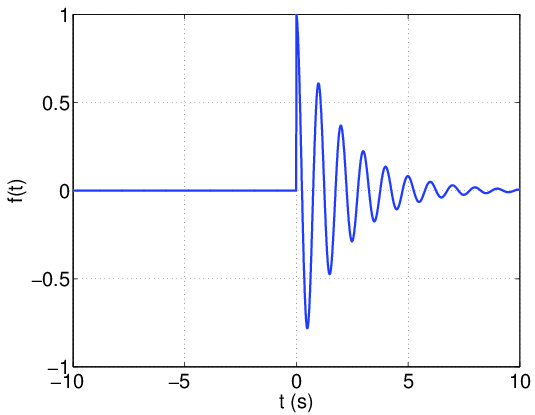
\includegraphics[width=3.7cm]{./Figuras/Causal}&
      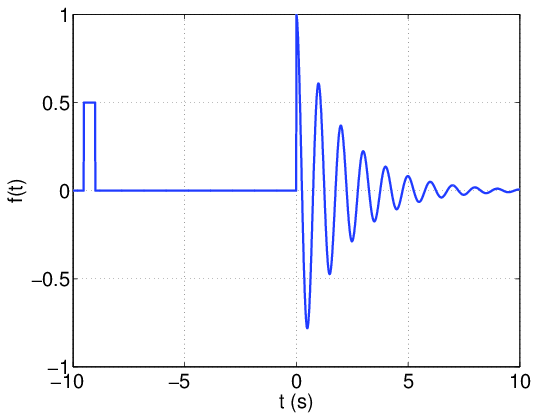
\includegraphics[width=3.7cm]{./Figuras/NoCausal}&
      \includegraphics[width=3.7cm]{./Figuras/Anticausal}\\
      Causal & No causal & Anticausal
    \end{tabular}
  \end{figure}
\end{frame}

\begin{frame}
  \frametitle{Tipos de señales VII}
  \begin{itemize}
    \item <1-> Señales definidas en energía):
    \begin{itemize}
      \vspace{0.2cm}
      \item \alert{Energía de una señal}:
      \vspace{0.2cm}
      \begin{itemize}
        \item Continua: $\varepsilon_x=\int^\infty_{-\infty}|x(t)|^2 dt $
        \vspace{0.2cm}
        \item  Discreta: $\varepsilon_x=\sum^{\infty}_{n=-\infty}|x[n]|^2 $
      \end{itemize}
      \vspace{0.2cm}
      \item \alert{Señal de energía finita}:  $0<\varepsilon_x<\infty$
      \begin{itemize}
        \vspace{0.2cm}
        \item En general son señales limitadas en el tiempo con amplitud finita
        \item Se puede analizar su espectro con la Transformada de Fourier.
      \end{itemize}
      \vspace{-0.2cm}
    \end{itemize}
  \end{itemize}

  \begin{figure}
    \centering
    \footnotesize
    \begin{tabular}{@{\extracolsep{-8pt}}cc}
      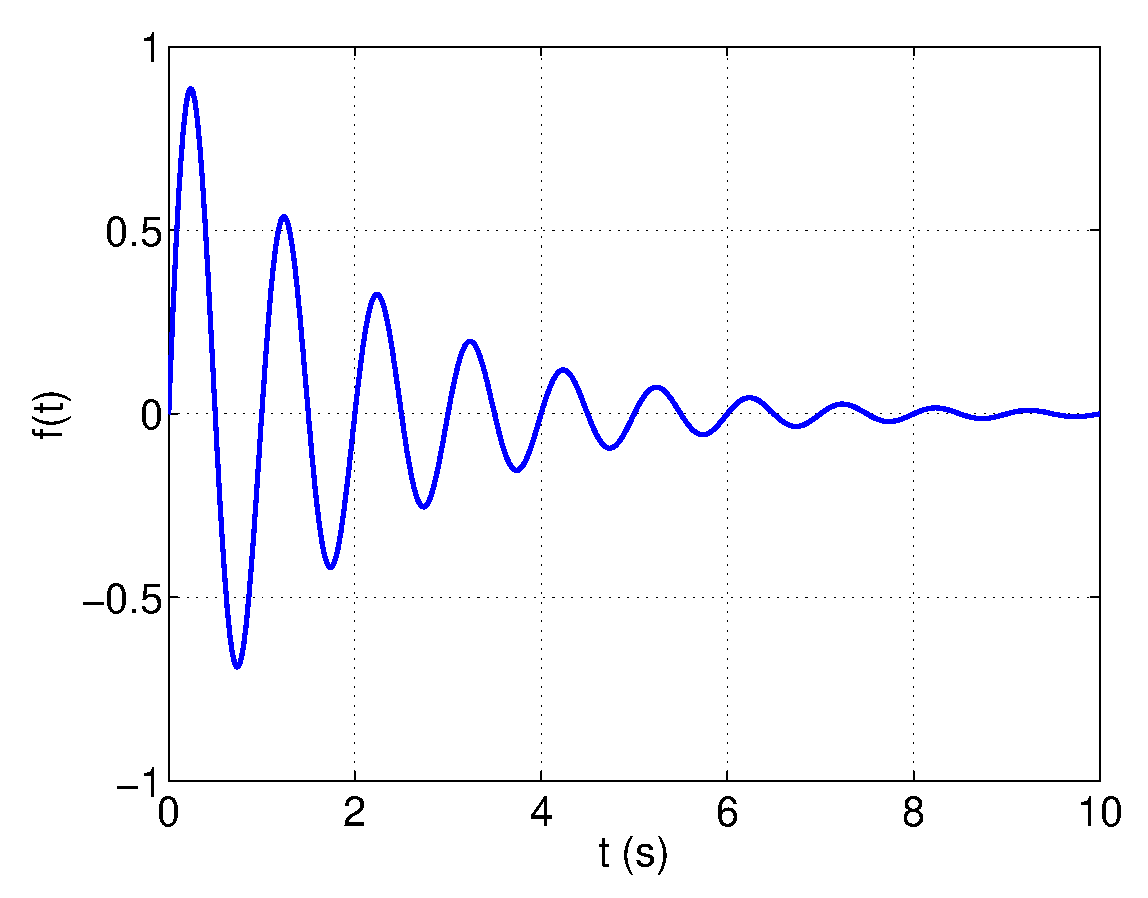
\includegraphics[width=4.5cm]{./Figuras/EnergiaF.eps}&
      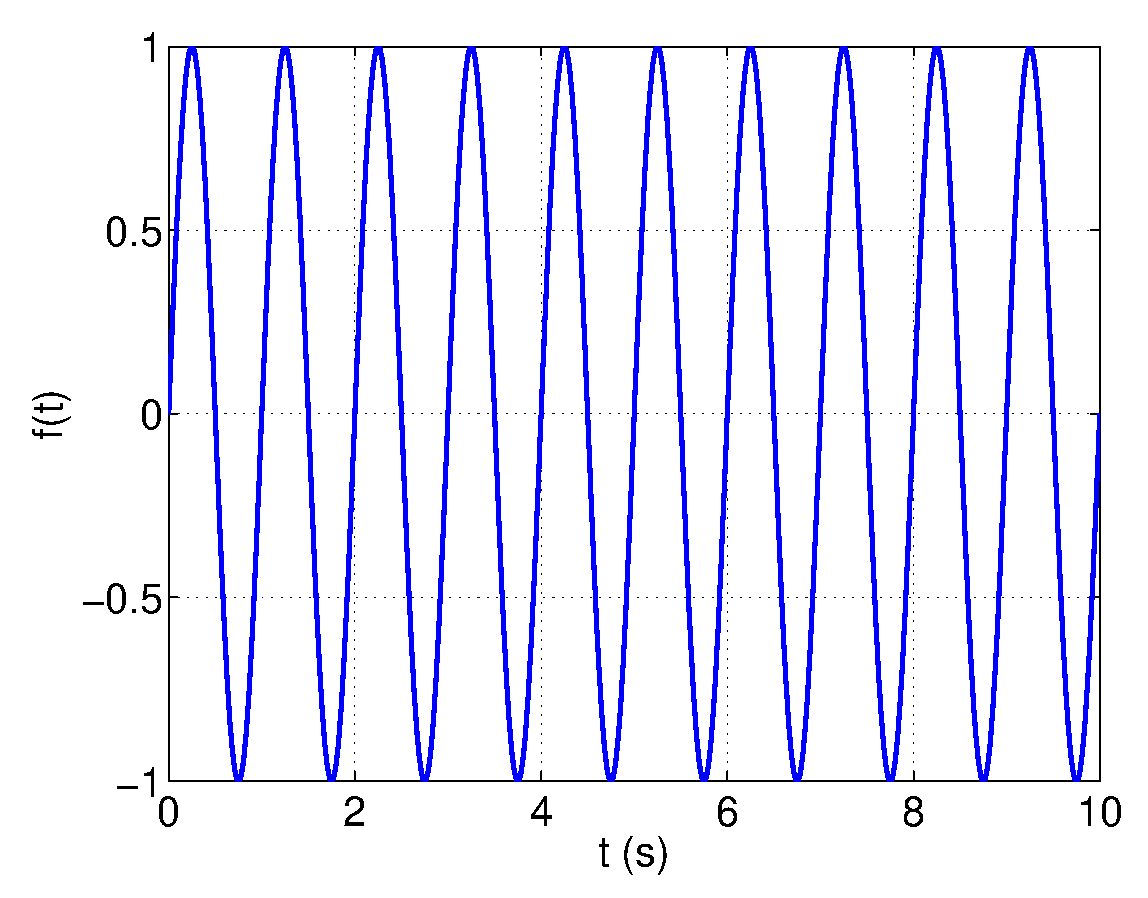
\includegraphics[width=4.5cm]{./Figuras/EnergiaI.eps}\\
      Energía finita & Energía infinita
    \end{tabular}
  \end{figure}
\end{frame}

\begin{frame}
  \frametitle{Tipos de señales VIII}
  \begin{itemize}
    \item <1-> Señales definidas en potencia:
    \begin{itemize}
      \vspace{0.2cm}
      \item \alert{Potencia media de una señal}:
      \vspace{0.2cm}
      \begin{itemize}
        \item Continua: $P_f=\lim_{T\rightarrow \infty} \frac{1}{T} \int^T_{-T}|x(t)|^2 dt $
        \vspace{0.2cm}
        \item  Discreta: $P_f=\lim_{N\rightarrow \infty} \frac{1}{2N+1}\sum^{N}_{n=-N}|x[n]|^2 $
      \end{itemize}
      \vspace{0.2cm}
      \item \alert{Señal de potencia media finita}:  $0<P_f<\infty$
      \begin{itemize}
        \vspace{0.2cm}
        \item En general son señales ilimitadas en el tiempo con amplitud finita.
      \end{itemize}
      \vspace{-0.4cm}
    \end{itemize}
  \end{itemize}

  \begin{figure}
    \centering
    \footnotesize
    \begin{tabular}{@{\extracolsep{-8pt}}cc}
      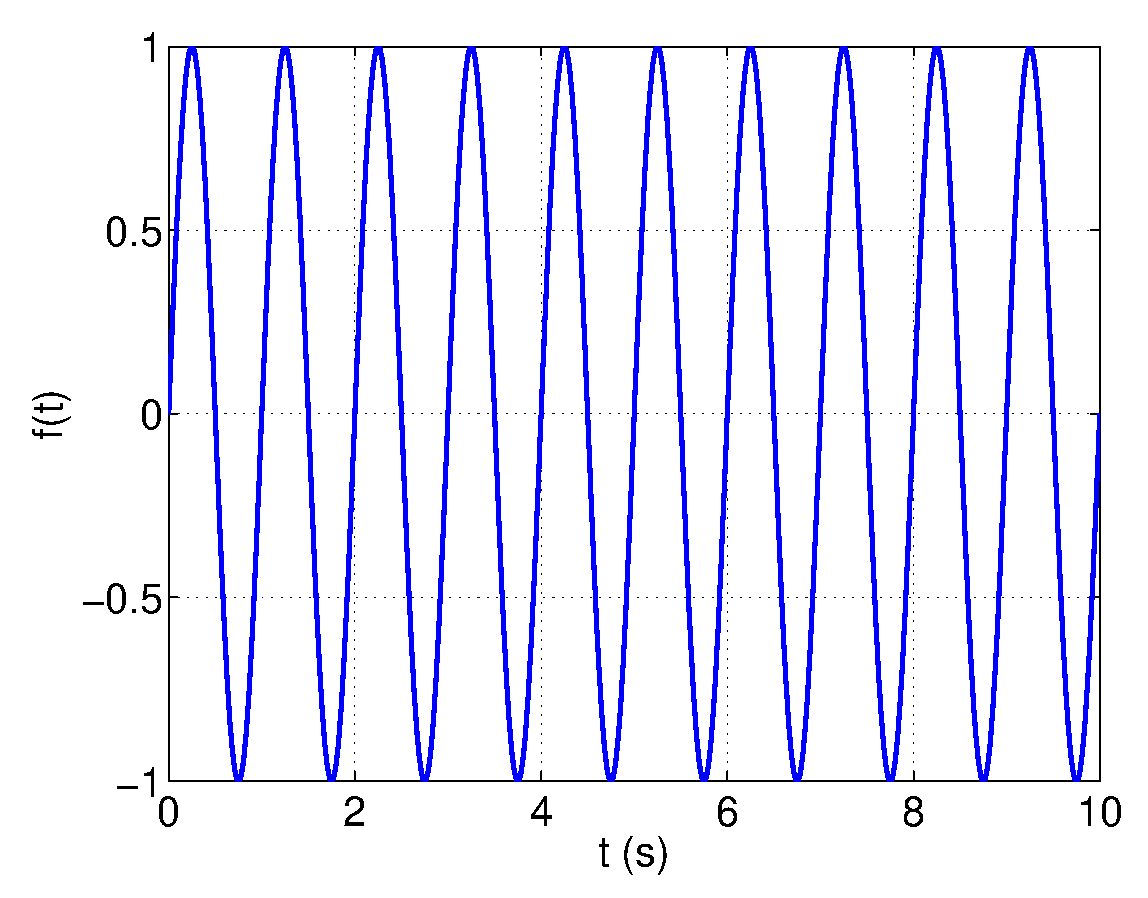
\includegraphics[width=4cm]{./Figuras/EnergiaI.eps}&
      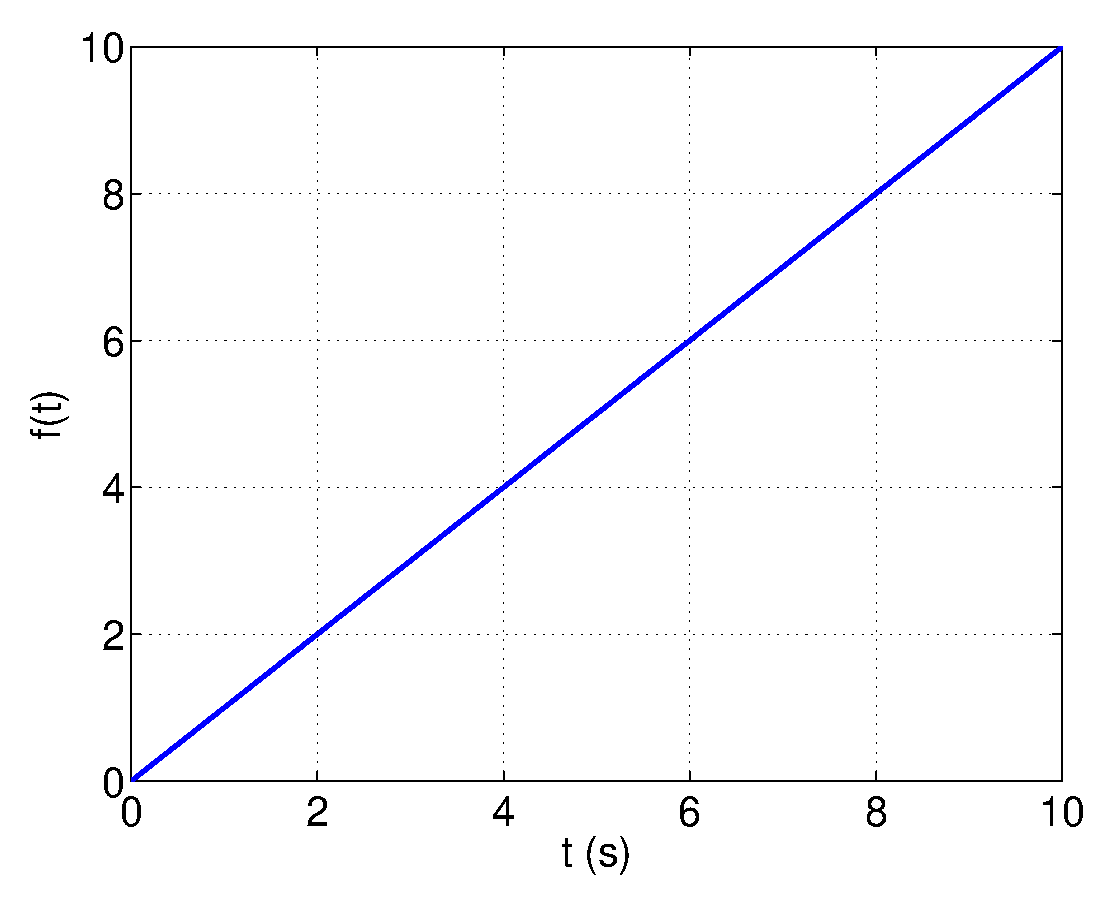
\includegraphics[width=3.8cm]{./Figuras/PotenciaI.eps}\\
      Potencia finita & Potencia infinita
    \end{tabular}
  \end{figure}

  \scriptsize \color{gray} \textit{Señales que no son de energía ni de potencia media finita son en general ilimitadas en el tiempo y/o amplitud.}
\end{frame}

% % %%%%%%%%%%%%%%%%%%%%%%%%%%%%%%%%%%%%%%%%%%%%%%%%%%%%%%

\begin{frame}
  \frametitle{Tipos de señales IX}
  \vspace{-0.1cm}
  \small
  \begin{itemize}
    \item \alert{Señal compleja}:  $x(\cdot) \in \mathbb{C}$
    \vspace{0.1cm}
    \begin{itemize}
      \footnotesize
      \item Se representa mediante dos funciones reales que contengan la parte real e imaginaria, o la fase y la amplitud\\ [1ex]
      \hspace{0.4cm}$x(\cdot)=\mathrm{Re}\{x(\cdot)\}+j \cdot \mathrm{Im}\{ x(\cdot)\}=|x(\cdot)| \mathrm{e}^{j \cdot \mathrm{arg} x(\cdot)}$
      \vspace{0.2cm}
      \begin{columns}[T]
        \begin{column}{4.75cm}
          \footnotesize\centering
          Parte real e imaginaria
          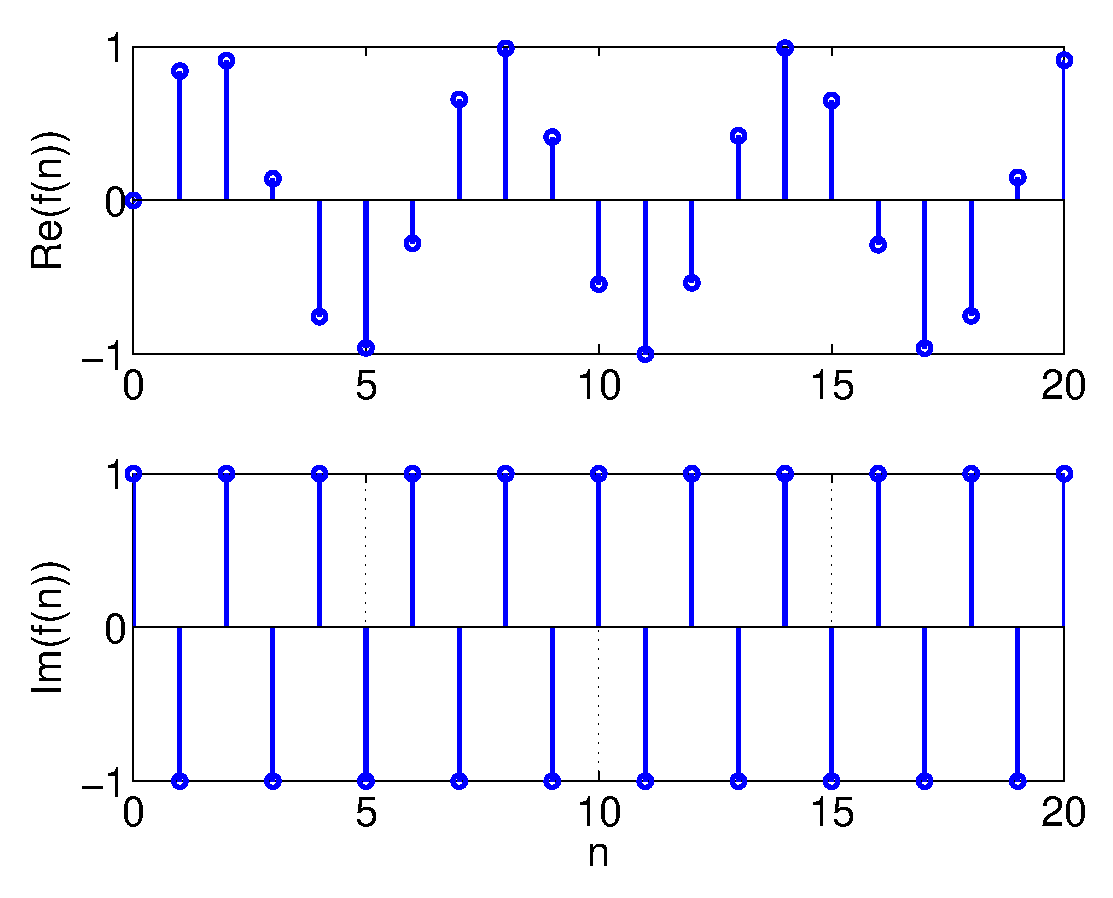
\includegraphics[width=3.5cm]{Figuras/ReIm.eps}
          $\begin{aligned}
            \mathrm{Re}(x(\cdot)) &= |x(\cdot)| \mathrm{cos}(\mathrm{arg}~x(\cdot) ) \\
            \mathrm{Im}(x(\cdot)) &= |x(\cdot)| \mathrm{sin}(\mathrm{arg}~x(\cdot))
          \end{aligned}$
        \end{column}
        \hspace{-1.2cm} \begin{column}{4.5cm}
          \footnotesize\centering
          Módulo y argumento
          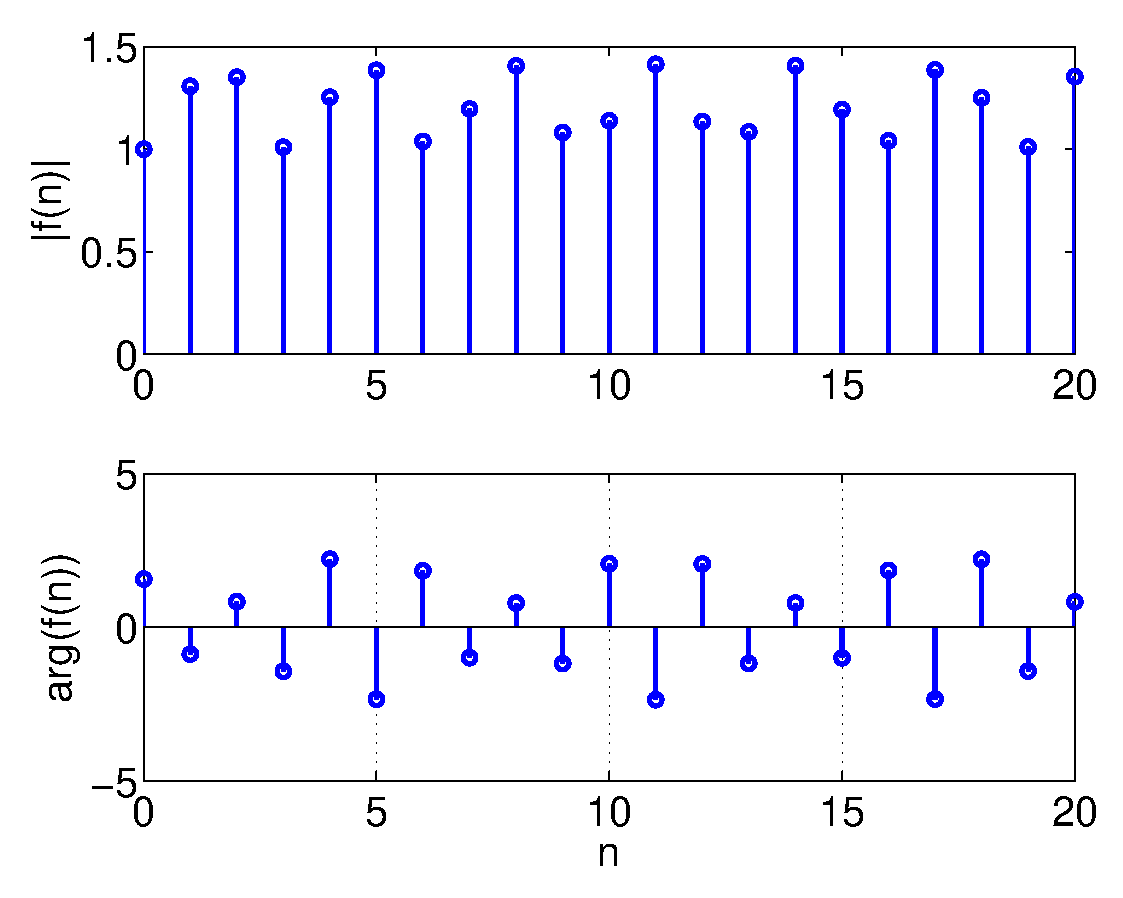
\includegraphics[width=3.5cm]{Figuras/ModArg.eps}\\
          $\begin{aligned}
            |x(\cdot)|            &= \sqrt{\mathrm{Re}\{x(\cdot)\}^2+\mathrm{Im}\{x(\cdot)\}^2} \\
            \mathrm{arg} x(\cdot) &= \arctan \frac{\mathrm{Im}\{x(\cdot)\}}{\mathrm{Re}\{x(\cdot)\}}
        \end{aligned}$
        \end{column}
      \end{columns}
    \end{itemize}
  \end{itemize}

  \vspace{-0.1cm}

  \scriptsize \color{gray} \textit{Series y Transformadas de Fourier. En teoría de la comunicación modelan señales  que transmiten información en fase y amplitud}

\end{frame}

% %%%%%%%%%%%%%

\begin{frame}
  \frametitle{Tipos de señales X}
  \vspace{-0.1cm}
  \small
  \begin{itemize}
    \item \alert{Señal reales}:$x(\cdot) = x^*(\cdot)$\\
    \vspace{0.1cm}
    \color{gray} $a(t)+j\cdot b(t)=a(t)-j \cdot b(t) \rightarrow b(t)=0$ \color{black}\\
    \item \alert{Señal imaginarias}: $x(\cdot) = -x^*(\cdot)$
    \vspace{0.1cm}
    \color{gray} $a(t)+j\cdot b(t)=-(a(t)-j \cdot b(t)) \rightarrow a(t)=0$ \color{black}\\
    \item \alert{Señal hermítica}:  $x(\cdot) = x^*(-\cdot)$
    \vspace{0.1cm}
    \color{gray} $a(t)+j\cdot b(t)=a(-t)-j \cdot b(-t) \rightarrow a(t)$ Par, $b(t)$ Impar \color{black}
    \item \alert{Señal antihermítica}: $x(\cdot) = -x^*(-\cdot)$\\
    \vspace{0.1cm}
    \color{gray} $a(t)+j\cdot b(t)=-(a(-t)-j \cdot b(-t)) \rightarrow a(t)$ Impar, $b(t)$ Par \color{black}
    \\ \vspace{0.2cm}
    con $^*$ conjugado.
  \end{itemize}

  \vspace{-0.3cm}
  \rule{10cm}{0.4pt}
  \vspace{0.2cm}\\
  \color{olivegreen}{Vamos a trabajar con señales: 1D (2D) escalares, continuas y discretas, analógicas y muestreadas, deterministas y aleatorias, periódicas y aperiódicas, reales y complejas.}

\end{frame}


%%%%%%%%%%%%%%%%%%%%%%%%%%%%%%%%%%%%%%%%%%%%%%

\begin{frame}
	\frametitle{Señales básicas: Impulso}
	
	\begin{itemize}
        \item \alert{Continuo ($\delta$ de Dirac):} {\scriptsize \hspace{1cm}$\delta(t)=\left \{ \begin{array}{l} \infty \:\: \: \:t=0\\0 \:\: \:\: \forall t \neq0\end{array}\right .$}%
        \begin{columns}[c]
            \begin{column}{0.2\textwidth}\centering
                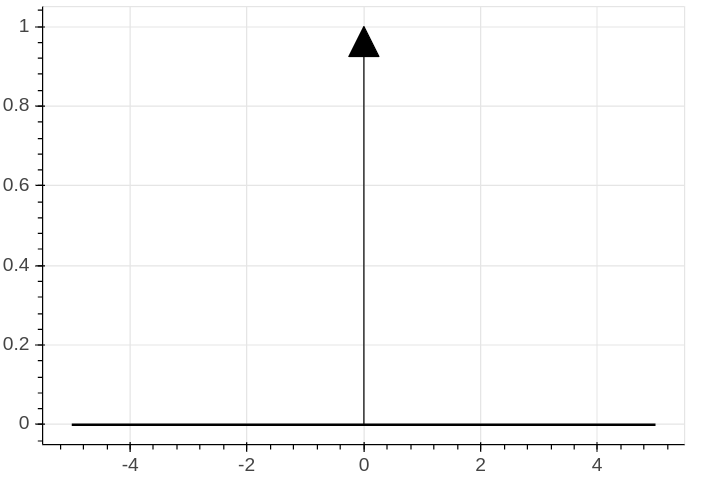
\includegraphics[width=4cm]{./Figuras/dirac}\\%
            \end{column}
            \hspace{0.3cm}
            \begin{column}{0.65\textwidth}
                {\scriptsize
                \begin{itemize}
                    {\scriptsize
                    \vspace{0.1cm}
                    \item Es un funcional:\\ \vspace{0.1cm}
                    $\int_{-\infty}^{\infty} f(t)\delta(t)dt=f(0)$\hspace{0.2cm}\color{olivegreen}$\int_{-\infty}^{\infty} f(t)\delta(t-t_0)dt=f(t_0)$\color{black}\\
                    \item Algunas propiedades:
                    $\int_{t_1}^{t_2} f(t)\delta(t-t_0)dt=\left\{\! \!\begin{array}{l}f(t_0)  \:\:\: t_1\!<t_0\!<t_2 \\ 0 \:\:\: c.c.    \end{array}\right .$
                    $\forall a\neq 0 \Rightarrow \delta(at)=\frac{\delta(t)}{|a|}$
                    $(x \ast \delta)(t) = \int_{-\infty}^\infty x(\tau)\delta(t-\tau)d\tau=x(t)$\\
                }\end{itemize}
                \vspace{0.2cm}
                \vspace{0.2cm}
            }\end{column}
        \end{columns}
        \vspace{-0.4cm}
        \item \alert{Discreto ($\delta$ de Kronecker):} {\scriptsize \hspace{0.5cm}$\delta(n)=\left \{ \begin{array}{l} 1\:\: \: \:n=0\\0 \:\: \:\: \forall n \neq0\end{array}\right .$}
        \begin{columns}[c]
            \begin{column}{0.22\textwidth}{\scriptsize
                \centering
                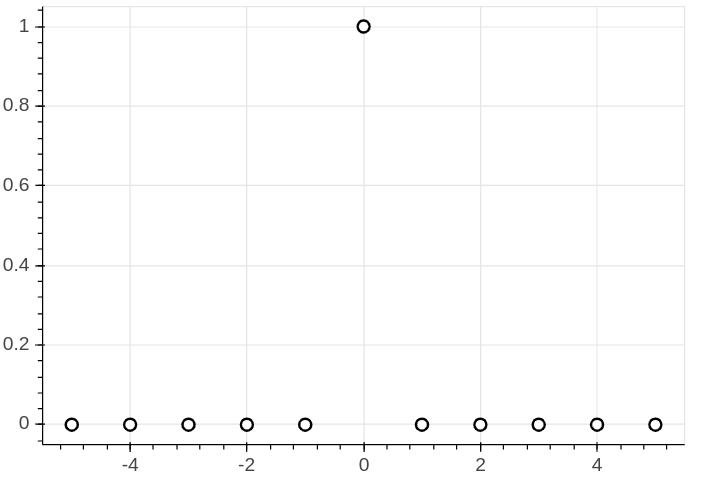
\includegraphics[width=4cm]{./Figuras/kronecker}\\%
            }\end{column}
            \begin{column}{0.65\textwidth}{\scriptsize
                \hspace{1.5cm}\color{olivegreen}$x[n]=\sum_{k=-\infty}^{\infty} x[k]\delta[k-n]$\color{black}\\
                \vspace{0.4cm}
                \hspace{1.5cm}$(x\! \ast\! \delta)[n] \!=\! \sum_{k=-\infty}^\infty x[k]\delta[n-k]=x[n]$
            }\end{column}
        \end{columns}
    \end{itemize}
\end{frame}
	
%%%%%%%%%%%%%%%%%%%%%%%%%%%%%%%%%%%%%%%%%%%%%%

\begin{frame}
\frametitle{Señales básicas: Escalón unitario}
  \begin{itemize}
    \begin{columns}[c]
        \begin{column}{7.0cm}
        
        \item \alert{Continuo:} $u(t)=\left \{ \begin{array}{l} 0 \:\: \: \:t<0\\1 \:\: \:\:  t \ge 0\end{array}\right .$

    \vspace{0.1cm}

        
        \small Relación con el impulso:

    \vspace{0.1cm}

    $\delta(t)=\frac{du(t)}{dt}$

    \vspace{0.1cm}

    $u(t)=\int _{-\infty} ^t \delta(\tau)d\tau$

    \vspace{0.1cm}

    Convolución: $(x \ast u)(t)=\int _{-\infty} ^t x(\tau)d\tau $
        
        \end{column}
    \hspace{-2.5cm}\begin{column}{5cm}
        \begin{figure}
    \centering
    \footnotesize
    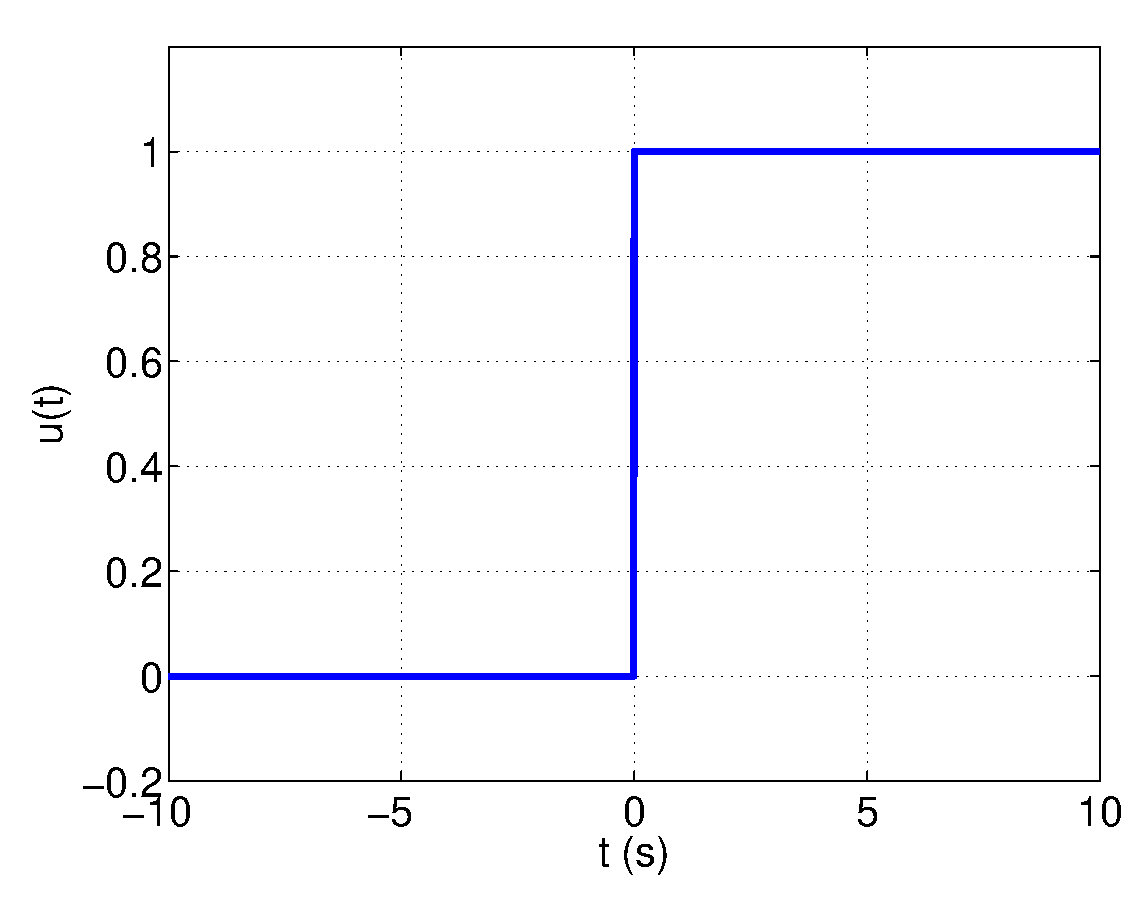
\includegraphics[width=4cm]{./Figuras/EscalonT.eps} 
    \end{figure}
        \end{column}
      \end{columns}
      
  \vspace{-0.2cm}

  \hspace{1cm}\begin{columns}[c]
      \begin{column}{6.0cm}
                      \item \alert{Discreto:}  $u[n]=\left \{ \begin{array}{l} 0\:\: \: \:n<0\\1 \:\: \:\:  n \ge 0\end{array}\right .$
      
              \vspace{0.2cm}
      
      \small Relación con el impulso:

  \vspace{0.2cm}

  $\delta[n]=u[n]-u[n-1]$

  \vspace{0.2cm}

  $u[n]=\sum _{k=-\infty} ^n \delta[k]$
      
      \vspace{0.2cm}

  Convolución: $(x\! \ast \! u)[n]\!=\!\sum _{k=-\infty} ^n x[k]$
      
      \end{column}
  \hspace{-1.5cm}\begin{column}{5cm}
      \begin{figure}
  \centering
  \footnotesize
  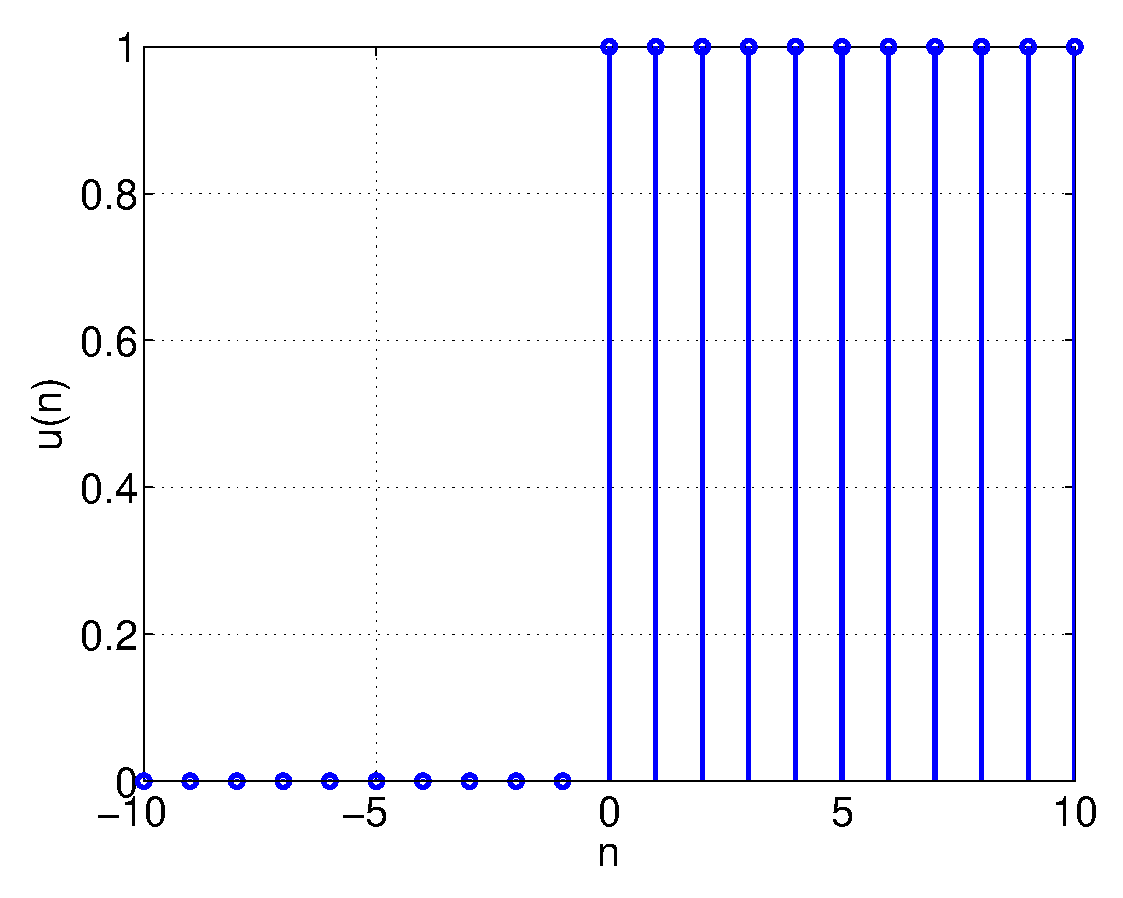
\includegraphics[width=4cm]{./Figuras/EscalonN.eps} 
  \end{figure}
      \end{column}
    \end{columns}
  \end{itemize}

  \small El producto de cualquier señal $x(\cdot)$ por $u(\cdot)$ produce una señal causal.
\end{frame}

%%%%%%%%%%%%%%%%%%%%%%%%%%%%%%%%%%%%%%%%%%%%%%%
	
	
\begin{frame}
\frametitle{Señales básicas: Rampa}

\begin{itemize}

\begin{columns}[c]
    \begin{column}{7.0cm}
        \item \alert{Continuo:} $r(t)=\left \{ \begin{array}{l} 0 \\ t \end{array}\begin{array}{l}t<0 \\ t \ge 0\end{array}\right .$

\vspace{0.1cm}

    
    \small Relación con el escalón:

\vspace{0.1cm}

$u(t)=\frac{dr(t)}{dt}$

\vspace{0.1cm}

$r(t)=\int _{-\infty} ^t u(\tau)d\tau$

\vspace{0.1cm}

    
    \end{column}
\hspace{-2.5cm}\begin{column}{5cm}
    \begin{figure}
\centering
\footnotesize
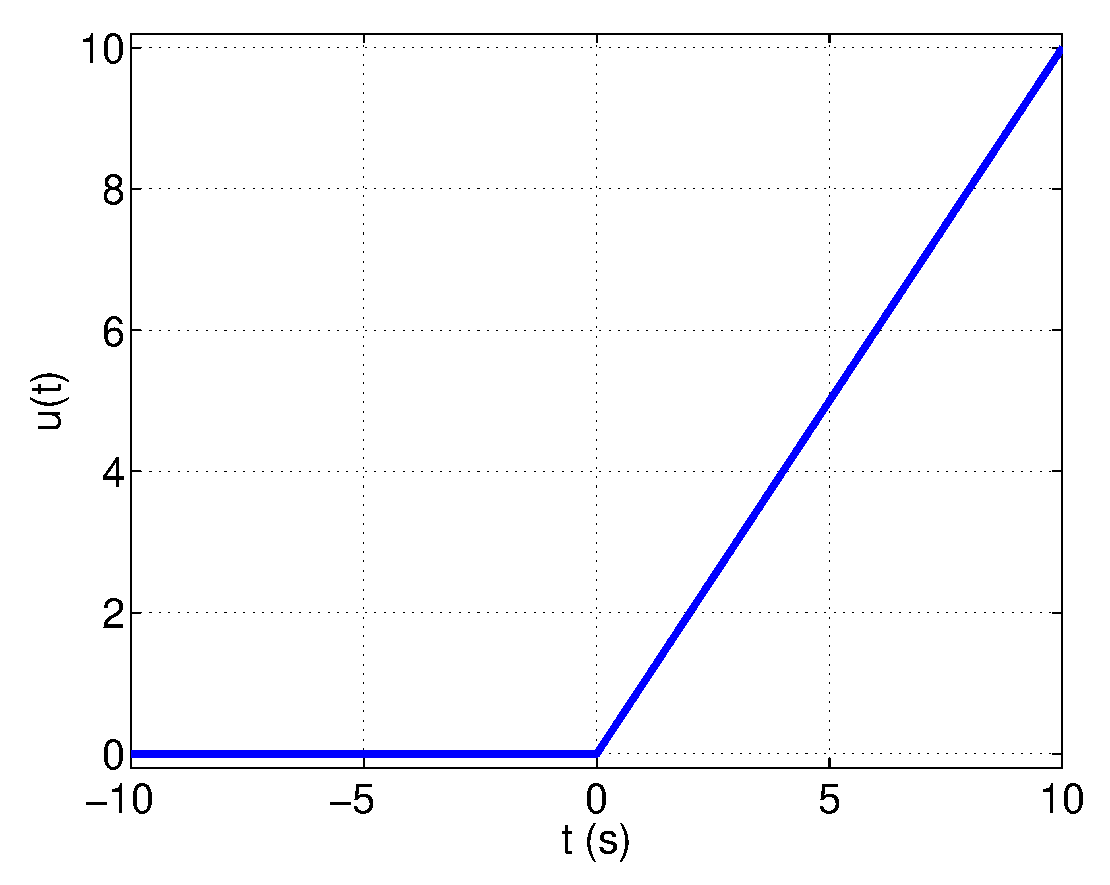
\includegraphics[width=4cm]{./Figuras/RampaT.eps} 
\end{figure}
    \end{column}
    \end{columns}
    
\vspace{-0.2cm}

\hspace{1cm}\begin{columns}[c]
    \begin{column}{6.0cm}
                    \item \alert{Discreto:}  $r[n]=\left \{ \begin{array}{l} 0 \\n+1\end{array}\begin{array}{l} n<0\\n \ge 0\end{array}\right .$
    
    
            \vspace{0.2cm}
    
    \small Relación con el escalón:

\vspace{0.2cm}

$u[n]=r[n]-r[n-1]$

\vspace{0.2cm}

$r[n]=\sum _{k=-\infty} ^n u[k]$
    
    \vspace{0.2cm}
    
    \end{column}
\hspace{-1.5cm}\begin{column}{5cm}
    \begin{figure}
\centering
\footnotesize
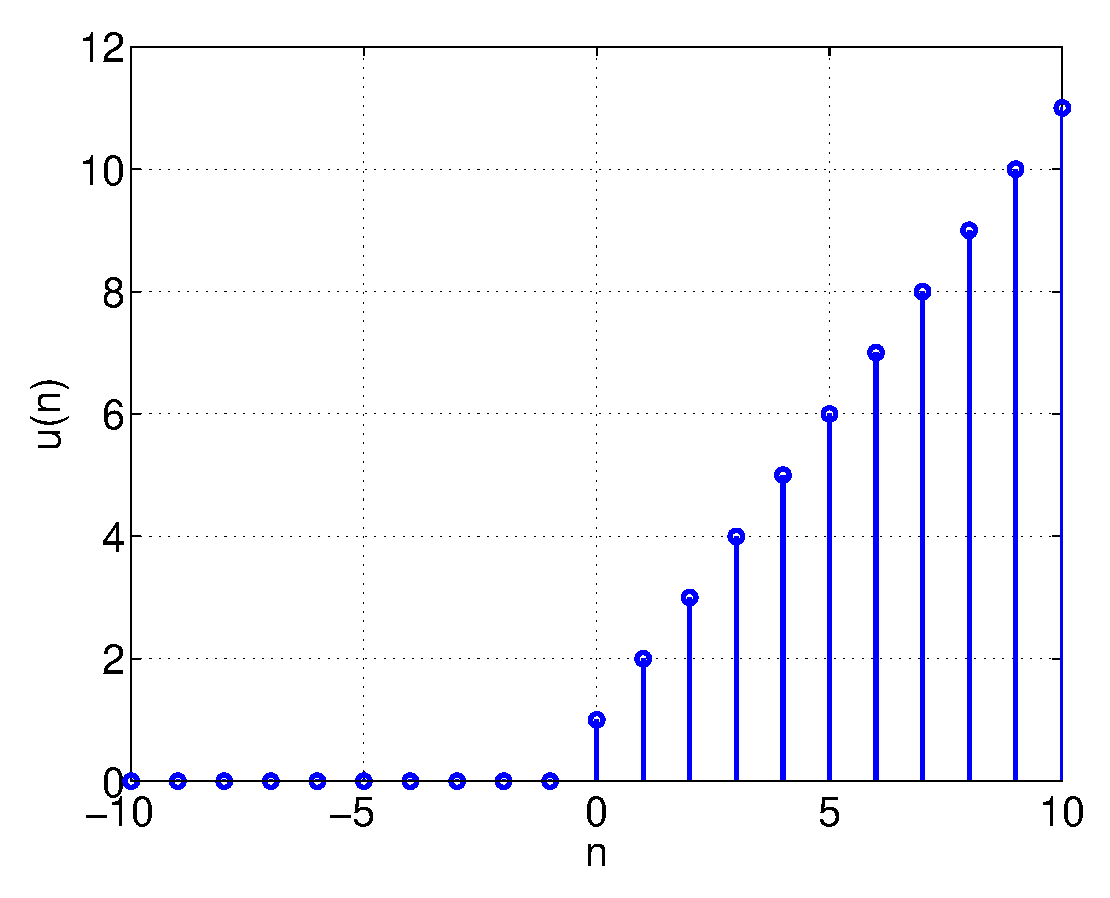
\includegraphics[width=4cm]{./Figuras/RampaN.eps} 
\end{figure}
    \end{column}
    \end{columns}


\end{itemize}


\end{frame}


%%%%%%%%%%%%%%%%%%%%%%%%%%%%%%%%%%%%%%%%%%%%%%

\begin{frame}\frametitle{Señales básicas: Pulsos}

    \begin{itemize}
        \begin{columns}[c]
            \begin{column}{5cm}
            \item \alert{Pulso rectangular}
                \vspace{0.3cm}
                $\Pi(t)=\left \{ \begin{array}{l} 1 \:\: \: \:|t| \le \frac{1}{2}\\0 \:\: \:\:  |t| > \frac{1}{2}\end{array}\right .$            
                \begin{figure}
                    \centering
                    \footnotesize
                    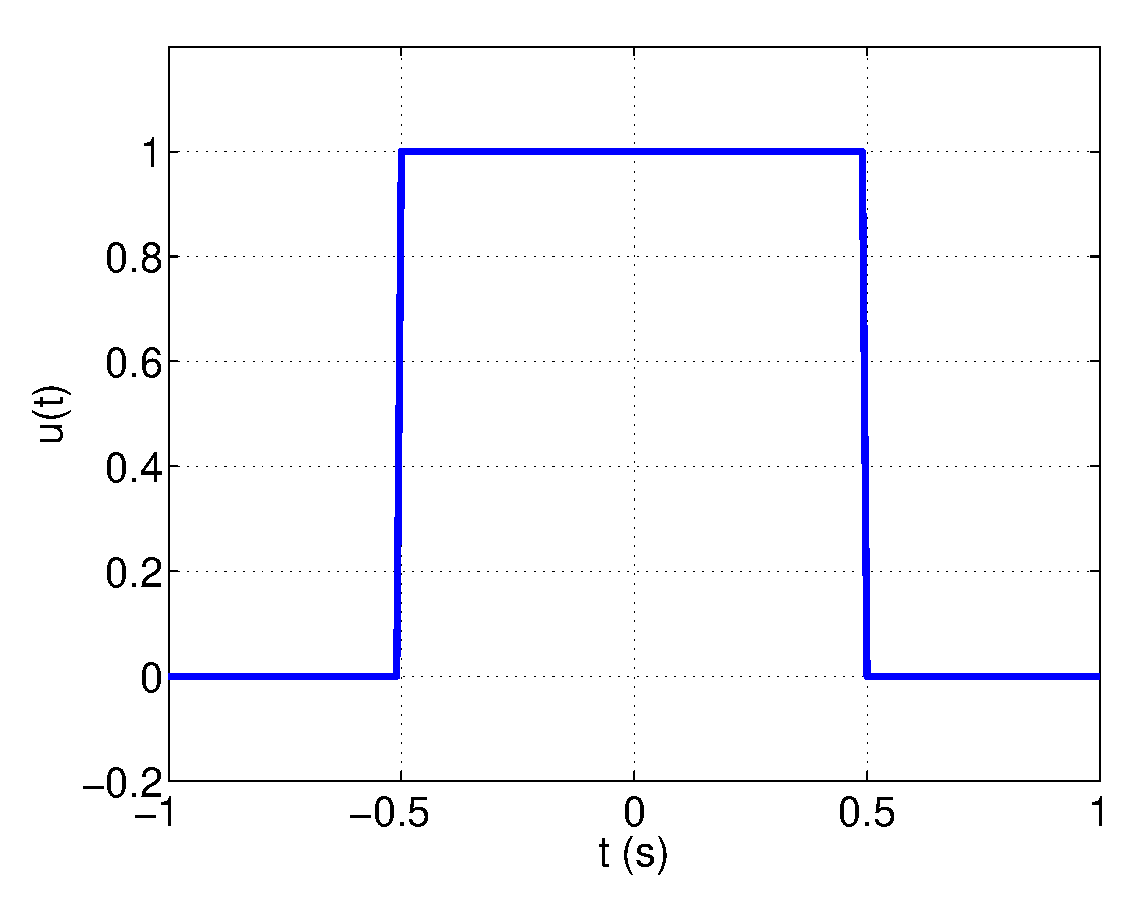
\includegraphics[width=5cm]{./Figuras/PulsoRect.eps} 
                \end{figure}
            \end{column}
            \begin{column}{5.cm}
                \item \alert{Pulso triangular}
                \vspace{0.3cm}
                $\Lambda(t)=\left \{\!\! \begin{array}{l} t+1 \:\: \: \:-1 \le t \le 0\\1-t \:\: \:\: \:\: \:\: \: 0 \le t \le 1\end{array}\right .$            
                \begin{figure}
                    \centering
                    \footnotesize
                    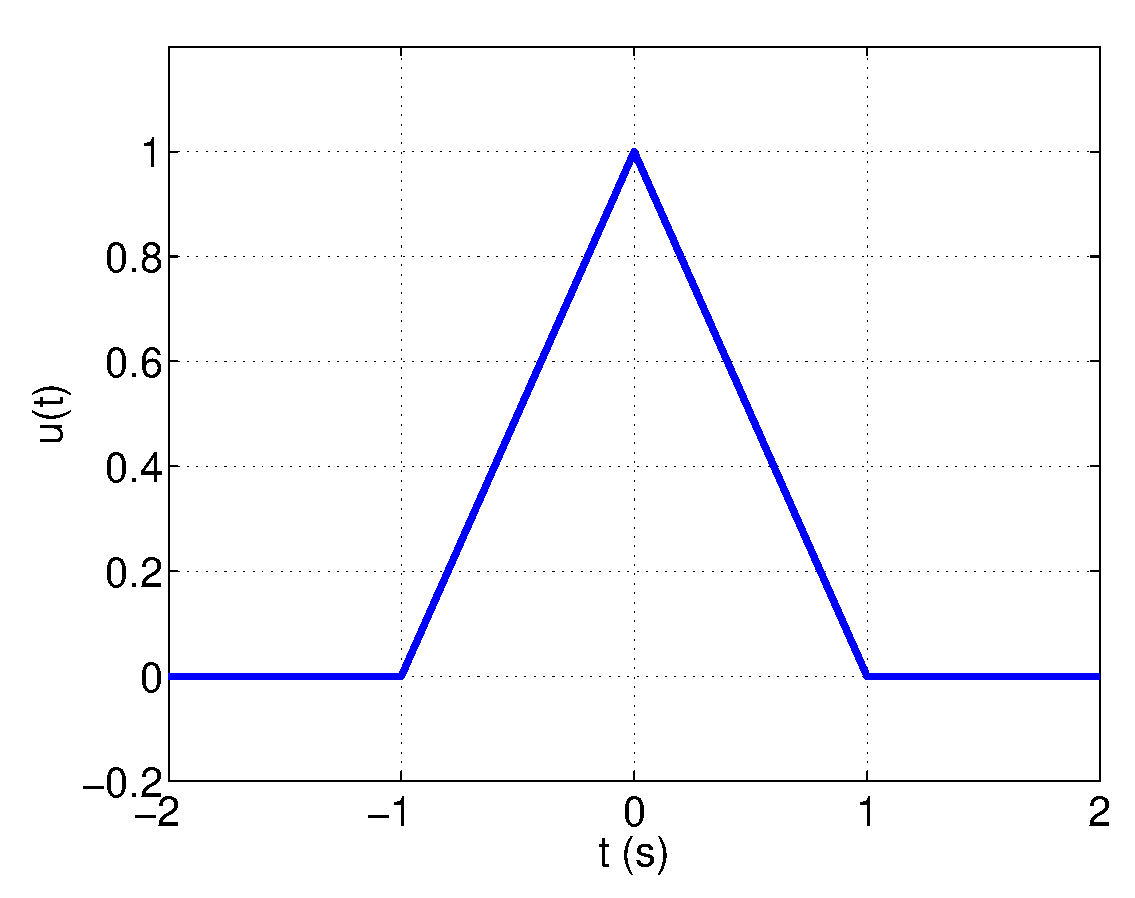
\includegraphics[width=5cm]{./Figuras/PulsoTri.eps} 
                \end{figure}
            \end{column}
        \end{columns}
    \end{itemize}
\end{frame}

%%%%%%%%%%%%%%%%%%%%%%%%%%%%%%%%%%%%%%%%%%%%%%%%%%%%%%
\begin{frame}
	\frametitle{Señales básicas: Exponencial Compleja}\centering
    \begin{itemize}
        \item \alert{Continua:} $x(t)=A\mathsf{e}^{\:j\omega t}$
		\begin{itemize}
            \item \color{blue}$x(t)=x(t+T)$\color{black}, con $T=\frac{1}{f}=\frac{2\pi}{\omega}$ \\
            \color{cyan}{\tiny $x(t+T)=A\mathsf{e}^{\:j\omega (t+\frac{2\pi}{\omega})}=A\mathsf{e}^{\:j(\omega t+2\pi)}=A\mathsf{e}^{\:j\omega t}\mathsf{e}^{\:j2\pi}=A\mathsf{e}^{\:j\omega t}$=x(t)}\color{black}
            \vspace{0.1cm}
            \item \color{blue}$\omega=2\pi f$ \color{black}es la frecuencia ($\omega$ rad/s, $f$ Hz)
            \vspace{0.1cm}
            \item \color{blue}$\omega_1\neq\omega_2 \Rightarrow x_1(t)\neq x_2(t)$\color{black}, para $0<\omega<\infty$
            \vspace{0.1cm}
        \end{itemize}
    \end{itemize}
    \begin{minipage}{0.25\textwidth}
        \centering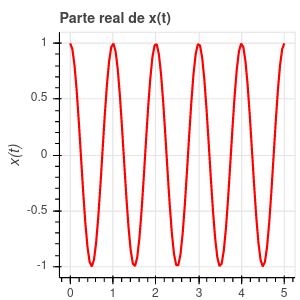
\includegraphics[width=\textwidth]{Figuras/exp_real.png}
    \end{minipage}
    \begin{minipage}{0.25\textwidth}
        \centering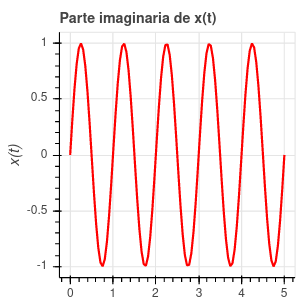
\includegraphics[width=\textwidth]{Figuras/exp_imag.png}
    \end{minipage}

    \begin{block}{{\scriptsize Fórmula de Euler}}\centering
        \scriptsize{$e^{j(\omega t+\phi)}=cos(\omega t+\phi)+j sin(\omega t+\phi)\Rightarrow \left\lbrace\begin{matrix}
            cos(\omega t+\phi)=\frac{e^{j(\omega t+\phi)}+e^{-j(\omega t+\phi)}}{2}\\
            sin(\omega t+\phi)=\frac{e^{j(\omega t+\phi)}-e^{-j(\omega t+\phi)}}{2j}\\
        \end{matrix}\right.$}
    \end{block}
\end{frame}


\begin{frame}
	\frametitle{Señales básicas: Exponencial Compleja}\centering

	\begin{itemize}
		\item \alert{Continua (Forma General):} $x(t)=C \mathsf{e}^{a t}$, con $C,a\in\mathbb{C}$
		\vspace{0.1cm}
		\begin{itemize}{\small
            \item $\left.\begin{matrix}C=|C|\mathsf{e}^{j\phi}\\a=r+j\omega\end{matrix}\right\rbrace \Rightarrow \color{blue}x(t)=|C| \mathsf{e}^{r t}\mathsf{e}^{\:j(\omega t+\phi)}\color{black}$
    %        \vspace{0.1cm}
            \item Sinusoidal multiplicada por exponencial
            \vspace{0.1cm}
            \item Decreciente ($r<0$), constante ($r=0$) o creciente ($r>0$)
            \vspace{0.1cm}
        }\end{itemize}
    \end{itemize}
    \begin{minipage}{0.25\textwidth}
        \centering\scriptsize{$r<0$}\\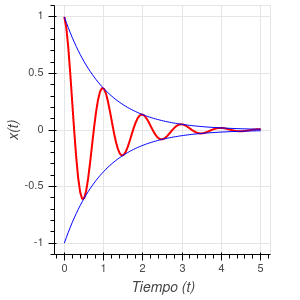
\includegraphics[width=\textwidth]{Figuras/exp_decreciente.png}
    \end{minipage}
    \begin{minipage}{0.25\textwidth}
        \centering\scriptsize{$r=0$}\\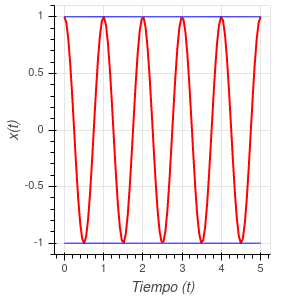
\includegraphics[width=\textwidth]{Figuras/exp_sin.png}
    \end{minipage}
    \begin{minipage}{0.25\textwidth}
        \centering\scriptsize{$r>0$}\\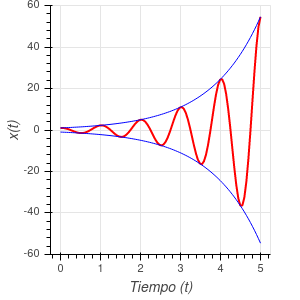
\includegraphics[width=\textwidth]{Figuras/exp_creciente.png}        
    \end{minipage}
    \begin{block}{{\scriptsize Fórmula de Euler}}\centering
        \scriptsize{$e^{j(\omega t+\phi)}=cos(\omega t+\phi)+j sin(\omega t+\phi)\Rightarrow \left\lbrace\begin{matrix}
            cos(\omega t+\phi)=\frac{e^{j(\omega t+\phi)}+e^{-j(\omega t+\phi)}}{2}\\
            sin(\omega t+\phi)=\frac{e^{j(\omega t+\phi)}-e^{-j(\omega t+\phi)}}{2j}\\
        \end{matrix}\right.$}
    \end{block}
\end{frame}


\begin{frame}
	\frametitle{Señales básicas: Exponencial Compleja}\centering
    \begin{itemize}
        \vspace{0.1cm}
		\item \alert{Discreta:} $x[n]=C \mathsf{e}^{j\omega n}$
		\begin{itemize}{\small
            \item \color{blue}$\omega=2\pi f$~\color{black} es la frecuencia en rad/muestra
            \vspace{0.1cm}
            \item \color{blue}$x[n]=x[n+N]$\color{black}, con $N=\frac{1}{f}=\frac{2\pi}{\omega}$ \color{red}sólo si \color{black}
            \vspace{0.1cm}
            \color{cyan}{\tiny $x[n+N]=C\mathsf{e}^{\:j\omega (n+N)}=C\mathsf{e}^{\:j(\omega n+\omega N)}=C\mathsf{e}^{\:j\omega n}\mathsf{e}^{\:j\omega N}=x[n]$\\
            \vspace{0.1cm}
            $\mathsf{e}^{\:j\omega N}=1\Rightarrow 2\pi f N=2\pi k \Rightarrow f=\frac{k}{N}$, para algún $N,k\in\mathbb{N}$\\
            Nota: $\frac{k}{N}$ es una fracción irreducible, en caso contrario $\frac{a}{b}=\frac{m\cdot k}{m\cdot N}=\frac{k}{N}$
            }\color{black}


            \vspace{0.1cm}
            \item \color{blue}$\omega_1\neq\omega_2 \Rightarrow x_1[n]\neq x_2[n]$\color{black}, \color{red}sólo para $0<\omega<2\pi\color{black}$\\
            \vspace{0.1cm}
            \color{cyan}{\scriptsize $\omega_k=\omega+2\pi k \Rightarrow$
            $C\mathsf{e}^{\:j(\omega + 2\pi k) n}=C\mathsf{e}^{\:j\omega n+j2\pi k n}=C\mathsf{e}^{\:j\omega n}\mathsf{e}^{\:j2\pi k n}=C\mathsf{e}^{\:j\omega n}$}\color{black}
            \vspace{0.1cm}
        }\end{itemize}
    \end{itemize}

    \begin{block}{{\scriptsize Fórmula de Euler}}
        \centering
        \scriptsize{$e^{j\omega n+\phi}=cos(\omega n+\phi)+j sin(\omega n+\phi)\Rightarrow \left\lbrace\begin{matrix}
            cos(\omega n+\phi)=\frac{e^{j(\omega n+\phi)}+e^{-j(\omega n+\phi)}}{2}\\
            sin(\omega n+\phi)=\frac{e^{j(\omega n+\phi)}-e^{-j(\omega n+\phi)}}{2j}\\
        \end{matrix}\right.$}
    \end{block}
\end{frame}


\begin{frame}
	\frametitle{Señales básicas: Exponencial Compleja}\centering
    \begin{itemize}{\scriptsize
        \vspace{0.1cm}
		\item \alert{Exponencial Discreta (sinusoidal):} $x[n]=C \alpha^n$, con $C,\alpha\in\mathbb{C}$
		\begin{itemize}{\scriptsize
            \item $\left.\begin{matrix}C=|C|e^{\phi}\\\alpha=|\alpha|e^{j\omega}\end{matrix}\right\rbrace \Rightarrow\color{blue}x(t)=|C||\alpha|^{n}e^{~j\omega n+\phi}\color{black}$
            \vspace{0.1cm}
            \item Decreciente ($0<\alpha<1$), constante ($\alpha=1$), o creciente ($\alpha>1$)
            \vspace{0.1cm}
        }\end{itemize}
    }\end{itemize}
    \begin{minipage}{0.25\textwidth}
        \centering\scriptsize{$0<|\alpha|<1$}\\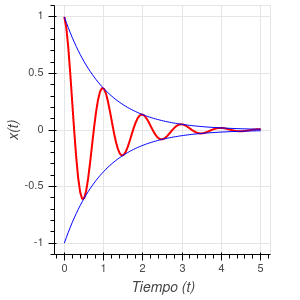
\includegraphics[width=\textwidth]{Figuras/exp_decreciente.png}
    \end{minipage}
    \begin{minipage}{0.25\textwidth}
        \centering\scriptsize{$|\alpha|=1$}\\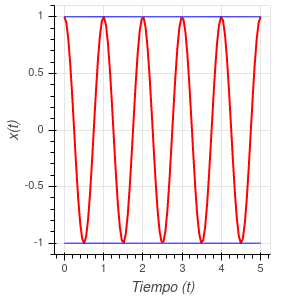
\includegraphics[width=\textwidth]{Figuras/exp_sin.png}
    \end{minipage}
    \begin{minipage}{0.25\textwidth}
        \centering\scriptsize{$|\alpha|>1$}\\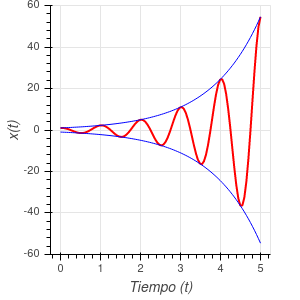
\includegraphics[width=\textwidth]{Figuras/exp_creciente.png}
    \end{minipage}

    \begin{block}{Fórmula de Euler}
        \centering
        \scriptsize{$e^{j\omega n+\phi}=cos(\omega n+\phi)+j sin(\omega n+\phi)\Rightarrow \begin{matrix}
            cos(\omega n+\phi)=\frac{e^{j\omega n+\phi}+e^{-j\omega n-\phi}}{2}\\
            sin(\omega n+\phi)=\frac{e^{j\omega n+\phi}-e^{-j\omega n-\phi}}{2}\\
        \end{matrix}$}
    \end{block}
\end{frame}



\begin{frame}
\frametitle{Señales básicas: muestreo, sinc, signo }

\vspace{-0.4cm}

\begin{itemize}



\begin{columns}[c]
    \begin{column}{4.5cm}
    
    \vspace{-0.8cm}
    
    \item \alert{Muestreo}

\vspace{0.3cm}

        $Sa(t)=\left \{ \begin{array}{l} \frac{sin(t)}{t} \:\: \: \:t \neq 0\\1 \:\: \:\: \:\: \:\: \:\: \:t=0\end{array}\right .$
        
            \item \alert{Sinc}

\vspace{0.3cm}

        $sinc(t)=\left \{\!\! \begin{array}{l} \frac{sin(\pi t)}{\pi t} \:\: \: \: t \ne 0 \\1 \:\: \:\:  \:\: \:\: \:\: \:\:  \: t=0\end{array}\right .$
    
    
    \vspace{0.7cm}
    
    
    \item \alert{Signo}

\vspace{0.3cm}

        $sgn(t)=\left \{\!\! \begin{array}{l} 1 \:\: \: \: \:\: \:\:t > 0 \\-1 \:\: \:\:   t<0 \\ 0  \:\: \:\:  \:\: \:\: t=0\end{array}\right .$


    
    \end{column}
\hspace{-0.5cm}	\begin{column}{4.5cm}
    
    \vspace{0.6cm}
            \begin{figure}
\centering
\footnotesize
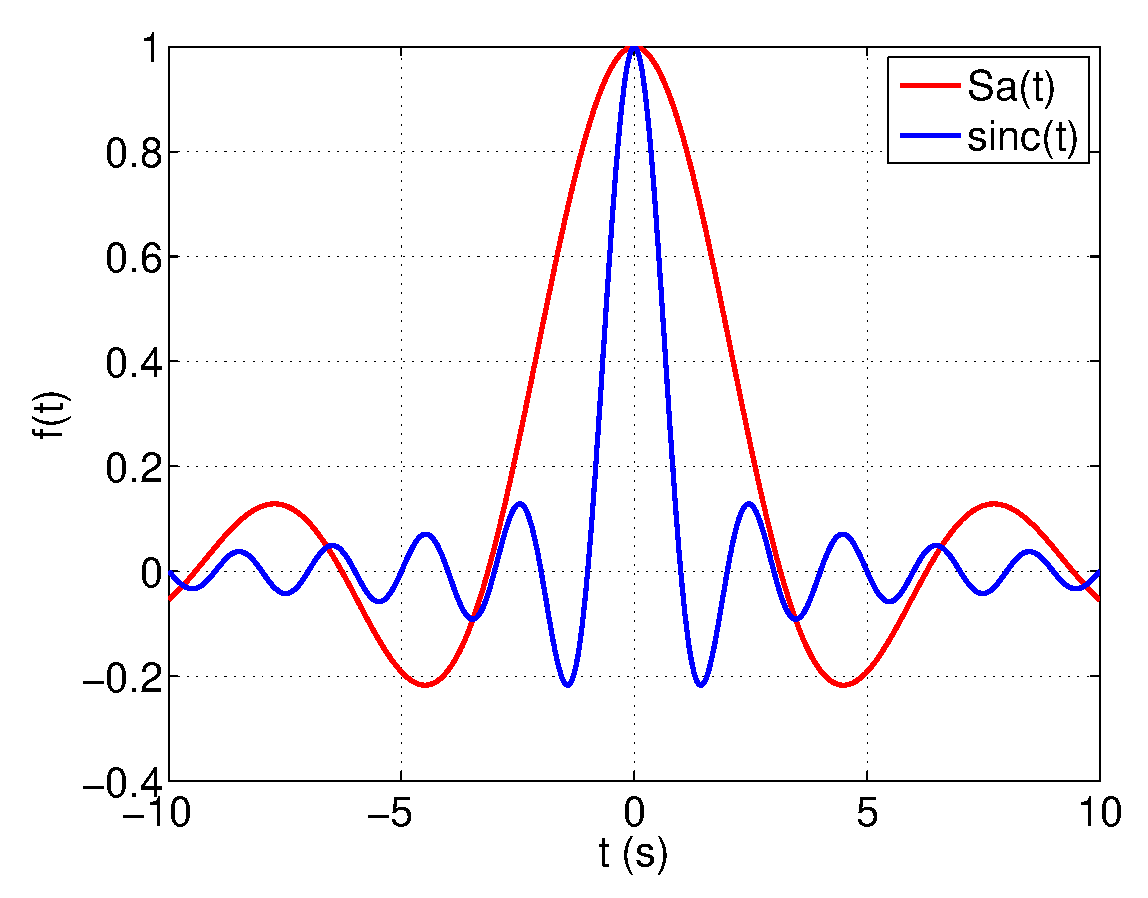
\includegraphics[width=4.5cm]{./Figuras/MuestreoSinc.eps} 
\end{figure}

            \begin{figure}
\centering
\footnotesize
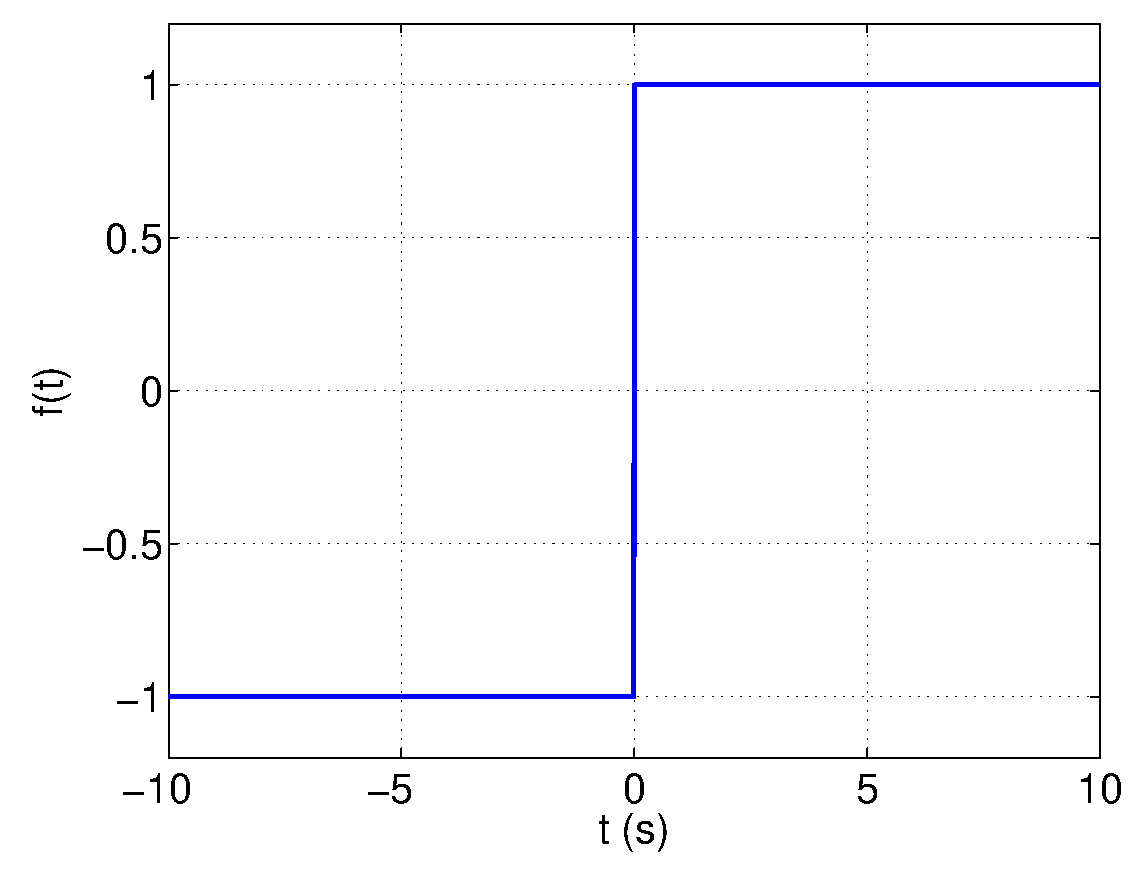
\includegraphics[width=4.5cm]{./Figuras/Signo.eps} 
\end{figure}

    
    \end{column}
    \end{columns}


\end{itemize}





\end{frame}

%%%%%%%%%%%%%%%%%%%%%%%%%%%%

\begin{frame}
\frametitle{Señales básicas: ondas  }

\begin{itemize}

\begin{columns}[c]
    \begin{column}{4.5cm}
    
    \item \alert{Onda cuadrada}

\vspace{0.3cm}

    
            
            \begin{figure}
\centering
\footnotesize
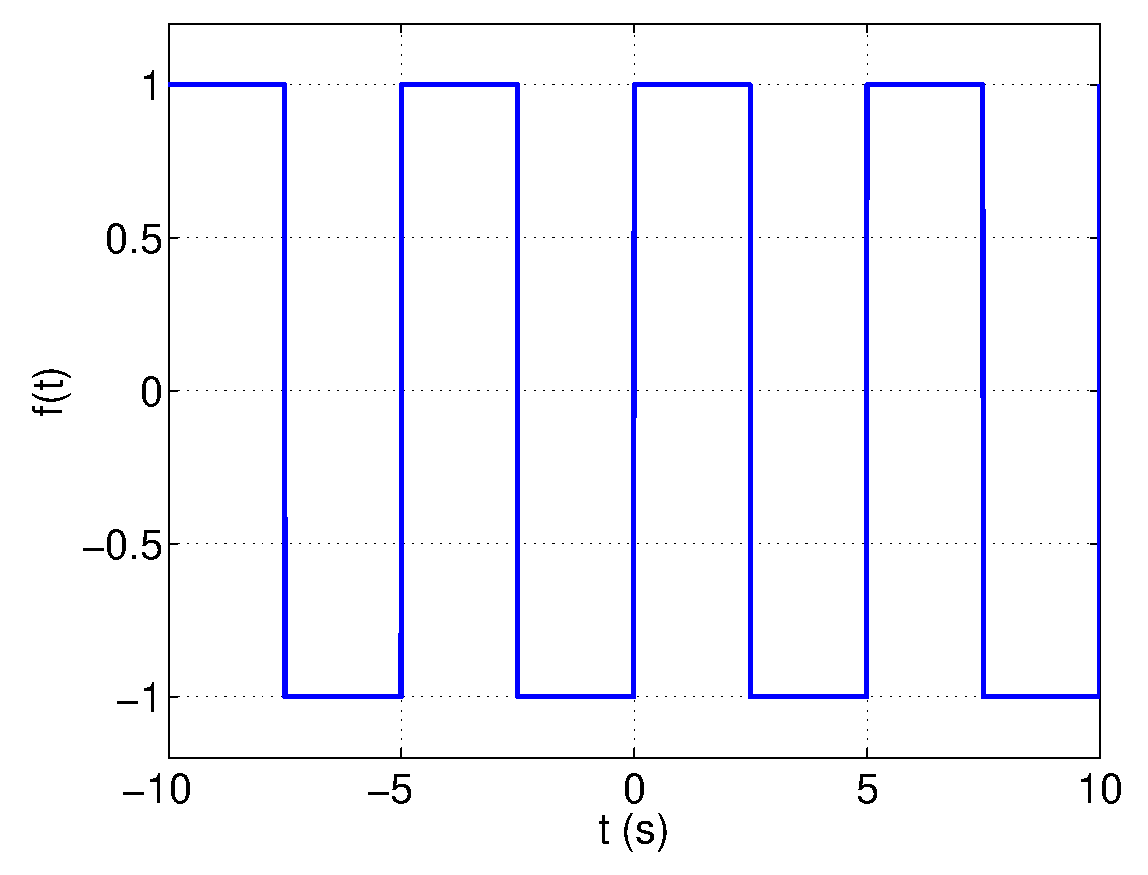
\includegraphics[width=4.5cm]{./Figuras/Square.eps} 

$T=5$
\end{figure}
    
    
    

    
    \end{column}
\hspace{-0.5cm}	\begin{column}{4.5cm}
    
        \item \alert{Onda triangular}

\vspace{0.3cm}




            \begin{figure}
\centering
\footnotesize
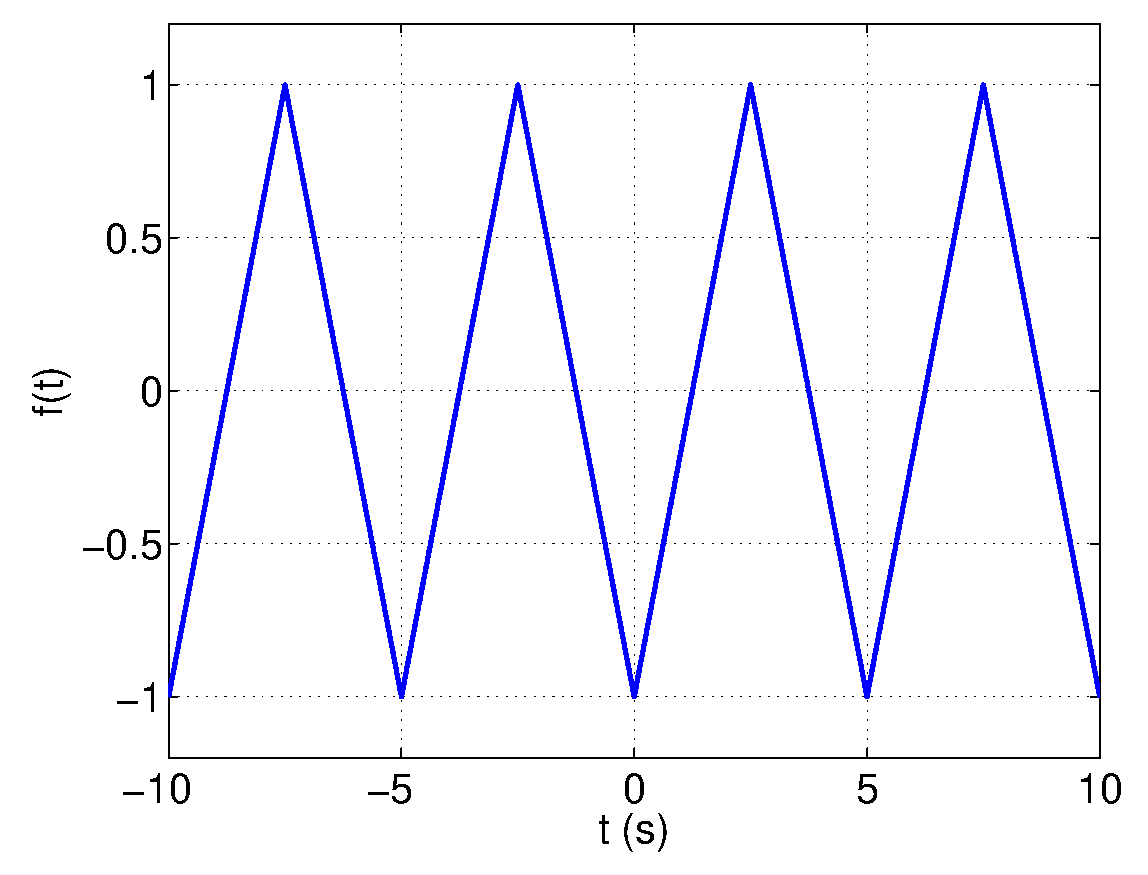
\includegraphics[width=4.5cm]{./Figuras/Triangular.eps} 

$T=5$
\end{figure}

    
    \end{column}
    \end{columns}


\end{itemize}

\end{frame}

\begin{frame}
\frametitle{Señales básicas: chirp  }

\begin{itemize}

\begin{columns}[c]

\hspace{-0.5cm}	\begin{column}{4.5cm}
    
        \item \alert{Chirp de variaci\'{o}n lineal}

\vspace{0.3cm}




\begin{figure}
    \centering
\footnotesize
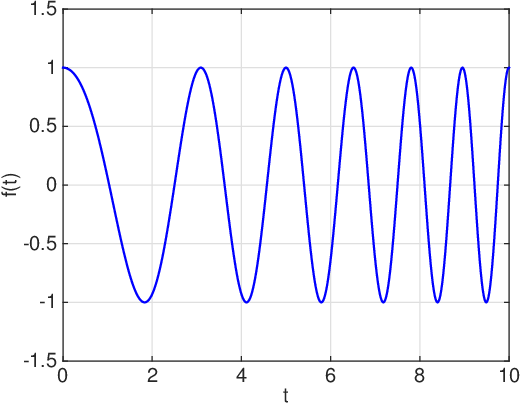
\includegraphics[width=4.5cm]{./Figuras/chirp} 

$f_{t=0}=0.2$ y $f_{t=10}=1$ 
\end{figure}

    
    \end{column}
    \end{columns}


\end{itemize}

\end{frame}


\begin{frame}\frametitle{Conceptos importantes}
  \begin{itemize}
    \item \alert{Definición de señal y sistema.}
    \item \alert{Clasificación de señales según sus características.}
    \begin{itemize}
      \item Analógica - Digital
      \item Periódica - Aperiódica
      \item Energía finita - Potencia finita - Señales no físicas
    \end{itemize}
    \item \alert{Señales básicas.}
    \begin{itemize}
      \item Impulso, Pulso (rectangular, triangular).
      \item Senoidales, Exponencial compleja.
      \item Exponencial real.
      \item Señales periódicas.
      \item Muestreo, sinc.
    \end{itemize}
  \end{itemize}
\end{frame}